\documentclass[10pt,a4paper,onecolumn]{article} % a4paper

\def\baselinestretch{1.35} % space it
\setlength{\parskip}{1.8mm plus4mm minus3mm}

\usepackage[pdftex]{graphicx}
\usepackage{amssymb}
\usepackage{amsmath}
\usepackage{amsthm}
\usepackage[square,comma,numbers,sort&compress]{natbib}
\usepackage{url}
\usepackage[font={small}, labelfont=bf]{caption} 


\newcommand{\f}{\on}

\usepackage{hyperref}


% The following parameters seem to provide a reasonable page setup.
\topmargin 0.0cm
\oddsidemargin 0.2cm
\textwidth 16cm
\textheight 21cm
\footskip 1.0cm

\renewcommand*\abstractname{Summary}

\usepackage{xcolor} 
\usepackage{epstopdf}% To incorporate .eps illustrations using PDFLaTeX, etc.
\usepackage{subfigure}% Support for small, `sub' figures and tables
\usepackage{multirow}
\usepackage{float}
\usepackage{environ}         % provides \BODY
\usepackage{etoolbox}        % provides \ifdimcomp
\usepackage{graphicx}        % provides \resizebox
\newlength{\myl}
\let\origequation=\equation
\let\origendequation=\endequation
\RenewEnviron{equation}{
  \settowidth{\myl}{$\BODY$}  % calculate width and save as \myl
  \origequation
  \ifdimcomp{\the\linewidth}{>}{\the\myl}
  {\ensuremath{\BODY}}                             % True
  {\resizebox{\linewidth}{!}{\ensuremath{\BODY}}}  % False
  \origendequation
}






%\theoremstyle{plain}% Theorem-like structures
\newtheorem{theorem}{Theorem}[section]

\newtheorem{lemma}[theorem]{Lemma}
\newtheorem{corollary}[theorem]{Corollary}
\newtheorem{proposition}[theorem]{Proposition}

%\theoremstyle{definition}
\newtheorem{definition}[theorem]{Definition}
\newtheorem{example}[theorem]{Example}

%\theoremstyle{remark}
\newtheorem{remark}{Remark}
\newtheorem{notation}{Notation}
\newcommand{\R}{\mathbb{R}}
\newcommand{\bs}{\boldsymbol}
\newcommand{\on}{\operatorname}



\title{A generalized closed-form maximum likelihood estimator}

\author{
Pedro L. Ramos$^1$, Eduardo Ramos$^2$, and Francisco A. Rodrigues$^2$, \\ and Francisco Louzada$^2$ \\  
\normalsize{$^{1}$ Facultad de Matemáticas, Pontificia Universidad Católica de Chile, Santiago, Chile} \\  
\normalsize{$^{2}$ Institute of Mathematics and Computer Science, University of S\~ao Paulo, S\~ao Carlos, Brazil}
}

\begin{document}

\maketitle

\begin{abstract}
The maximum likelihood estimator plays a fundamental role in statistics. However, for many models, the estimators do not have closed-form expressions. This limitation can be significant in situations where estimates and predictions need to be computed in real-time, such as in applications based on embedded technology, in which numerical methods can not be implemented. This paper provides a generalization in the maximum likelihood estimator that allows us to obtain the estimators in closed-form expressions under some conditions. Under mild conditions, the estimator is invariant under one-to-one transformations, strongly consistent, and has an asymptotic normal distribution. The proposed generalized version of the maximum likelihood estimator is illustrated on the Gamma, Nakagami, and Beta distributions and compared with the standard maximum likelihood estimator.
%to obtain closed-form expressions

\noindent \textbf{Keywords:} Closed-form estimators; Maximum Likelihood estimators; Generalized maximum likelihood estimator; generalized estimator.
\end{abstract}

%\begin{keywords}

%\end{keywords}

\section{Introduction}

%Statistics is widely concerned about proposing and improving inferential methods. 
Introduced by Ronald Fisher \citep{aldrich1997ra}, the maximum likelihood method is one of the most well-known and used inferential procedures to estimate the unknown parameters of a given distribution. 
Alternative methods to the maximum likelihood estimator (MLE) have been proposed in the literature, such as those based on statistical moments \citep{hosking1990moments}, percentile \citep{kao1,kao2}, product of spacings \citep{Cheng2}, or goodness of fit measures, to list a few. Although alternative inferential methods are popular nowadays, the MLEs are the most widely used due to their flexibility in incorporating additional complexity (such as random effects, covariates, censoring, among others) and their properties: asymptotical efficiency, consistent and invariance under one-to-one transformation. These properties are achieved when the MLEs satisfy some regularity conditions  \citep{2004-Bierens, 2006-Lehmann,redner1981note}.

It is now well established from various studies that the MLEs do not always return closed-form expressions for most common distributions. In these cases, numerical methods, such as Newton-Rapshon or its variants, are usually considered to find the values that maximize the likelihood function. Important variants of the maximum likelihood estimator, such as profile \citep{murphy2000profile}, pseudo \citep{gourieroux1984pseudo}, conditional \citep{andersen1970asymptotic}, penalized \citep{anderson1982penalized, firth1993bias} and marginal likelihoods \citep{cox1975partial}, have been presented to eliminate nuisance parameters and decrease the computational cost. Another important procedure to achieve the MLEs is the expectation-maximization (EM) algorithm \citep{dempster1977maximum}, which involves unobserved latent variables jointly with unknown parameters. The expectation and maximization steps also involve, in most cases, the use of numerical methods that may have a high computational cost. However, there is a need to use closed-form estimators to estimate the unknown parameters in many situations. For instance, in embed technology, small components need to compute the estimates without using maximization procedures, and in real-time applications, it is necessary to provide an immediate answer.

In the proposed study, we discuss a generalization for the maximum likelihood  method, which can, in many cases, be used to obtain closed-form expressions for the distribution parameters' estimators. Moreover, we propose conditions under which the proposed estimator is strongly consistent and asymptotic normal. Additionally, we show such conditions are greatly simplified for a general family of generalized maximum likelihood equations.

The proposed method is illustrated regarding the Gamma, Beta, and Nakagami distributions. In these cases, the standard ML does not have closed-form expressions, and numerical methods or approximations are necessary to find these distributions' solutions. Hence our approach does not require iterative numerical methods, and, computationally, the work required by using our estimators is less complicated than that required in ML estimators. The remainder of this paper is organized as follows. Section 2 presents the new generalized maximum likelihood estimator and its properties. Section 3 considers the application of the Gamma, Nakagami, and Beta distributions. Finally, Section 4 summarizes the study.


\section{Generalized Maximum Likelihood Estimator}

The method we propose here can be applied to obtain closed-form expressions for distributions with a given density $f(x\,;\,\bs\theta)$. In order to formulate the method, let $\Omega$ represent the sample space, let $\mathcal{X}$ represent the space of the data $x$, where $\mathcal{X}$ is equipped with a measure $\mu$, which can be either discrete or continuous, let $\Theta\subset \mathbb{R}^{s}$ be an open set containing the true parameter $\bs{\theta}_0$, to be estimated, and for each $x\in \mathcal{X}$ we let $\mathcal{A}_x\subset \mathbb{R}^{r}$, $0\leq r\leq s$ be an open set, possibly depending on $x$, containing  a fixed parameter $\bs{\alpha}_0$, which represents additional parameters which will be used during the procedure to obtain the estimators.

Now, suppose $X_1$, $X_2$, $\cdots$, $X_n$ are independent and identically distributed (iid) random variables, which can be either discrete or continuous, with a strictly positive density function  $f(x\,;\,\bs{\theta}_0)$. Then, given a function $g(x\,;\,\bs{\theta},\bs{\alpha})$ defined for $x\in \mathcal{X}$, $\bs{\theta}\in \Theta$ and $\bs{\alpha}\in \mathcal{A}_x$ we define the \textit{generalized maximum likelihood equations for $\bs{\theta}$ over the coordinates $(\theta_1,\cdots,\theta_{s-r},\bs{\alpha})$ at $\bs{\alpha}=\bs{\alpha}_0$} to be the set of equations
\begin{equation}\label{modified}
\begin{aligned}
&\frac{1}{n}\sum_{i=1}^n \frac{\partial}{\partial \theta_j}  \log\, g(X_i\,;\,\bs{\theta},\bs{\alpha}_0) = \on{E}_{\bs{\theta}}\left[\frac{\partial}{\partial \theta_j}  \log\, g(X_1\,;\,\bs{\theta},\bs{\alpha}_0)\right],\quad 1\leq j\leq s-r,\\ &\frac{1}{n}
\sum_{i=1}^n \frac{\partial}{\partial \alpha_j}  \log\, g(X_i\,;\,\bs{\theta},\bs{\alpha}_0)=\on{E}_{\bs{\theta}}\left[\frac{\partial}{\partial \alpha_j}  \log\, g(X_1\,;\,\bs{\theta},\bs{\alpha}_0)\right], \quad  1\leq j\leq r,
\end{aligned}
\end{equation}
as long as these partial derivatives exist and the expected values above are finite.

To see how the generalized likelihood equations generalize the maximum likelihood equations, note that, in case the equation $\int_{\mathcal{X}} f(x\,;\,\bs{\theta})\, d\mu =1$ can be differentiated under the integral sign we obtain $\int_{\mathcal{X}} \frac{\partial}{\partial \theta_j} f(x\,;\,\bs{\theta})\, d\mu =0$ for all $j$, in which case, letting $g(x\,;\,\bs{\theta})=f(x\,;\,\bs{\theta})$, it follows that the generalized maximum likelihood equations for $\bs{\theta}$ over the coordinates $(\theta_1,\cdots,\theta_s)$ are given by the equations
\begin{equation*}
\frac{1}{n}\sum_{i=1}^n \frac{\partial}{\partial \theta_j}  \log\, f(X_i\,;\,\bs{\theta}) = 0,\quad 1\leq j\leq s,
\end{equation*}
which coincide with the maximum likelihood equations. Note that the differentiation under the integral sign condition is a natural condition to impose, since it is universally used in order to prove the consistency and asymptotic normality of the maximum likelihood estimator.

From now on, our goal shall be that of giving conditions guaranteeing existence of solutions for the generalized maximum likelihood equations as well as conditions under which an obtained solution $\bs{\hat{\theta}}_n(X)$ of the generalized maximum likelihood equations is a consistent estimator for the true parameter $\bs{\theta}_0$, and is asymptotically normal. In order to formulate the result, given a fixed $\bs{\alpha}_0\in \Theta$ we denote
\begin{equation}\label{defh}
h_j(x\,;\,\bs{\theta}) = \frac{\partial}{\partial \beta_j}\log\, g \left(x\,;\,\bs{\theta},\bs{\alpha}_0\right) - \on{E}_{\bs{\theta}}\left[\frac{\partial}{\partial \beta_j}\log\, g \left(X_1\,;\,\bs{\theta},\bs{\alpha}_0\right)\right]
\end{equation}
for all $x$, $\bs{\theta}$ and $j$, where $(\beta_1,\cdots,\beta_s)=(\theta_1,\cdots,\theta_{s-r},\alpha_1,\cdots,\alpha_r)$. Moreover, we let $J(\bs{\theta})=\left(J_{i,j}(\bs{\theta})\right)\in M_{s}(\mathbb{R})$ and $K(\bs{\theta})=\left(K_{i,j}(\bs{\theta})\right)\in M_{s}(\mathbb{R})$, be defined by
 \begin{equation}\label{eqj}
 \begin{aligned}J_{i,j}(\bs{\theta})&=
 \on{E}_{\bs{\theta}} \left[-\frac{\partial}{\partial\theta_j}\, h_i(X_1\, ;\, \bs{\theta})\right]\mbox{ and}\\
 K_{i,j}(\bs{\theta}) &=  \on{cov}_{\bs{\theta}} \left[h_i(X_1\, ;\, \bs{\theta}),\,  h_j(X_1\, ;\, \bs{\theta})\right],
 \end{aligned}
 \end{equation}
 for all $1\leq i\leq s$ and $1\leq j\leq s$. These matrices shall play the role that the Fisher information matrix $I$ plays in the classical maximum likelihood method.
 %For instance if $r=0$ then, $I$, $J$ and $K$ coincide.

In the following we prove a result regarding the consistence of the estimator $\bs{\hat{\theta}}_n(X)$ defined above, for an arbitrary probability density function $f$.

\begin{theorem}\label{coprinc} Denote $\bs{X}=\left(X_1, X_2, \cdots, X_n\right)$, where $X_1$, $\cdots$, $X_n$ are iid with density $f(x\,;\,\bs{\theta}_0)$ and suppose:
\begin{itemize}

\item[(A)]  $J(\bs{\theta}_0)$ and $K(\bs{\theta}_0)$, as defined in (\ref{eqj}), exist and $J(\bs{\theta}_0)$ is invertible.
\item[(B)] $h_j(x\, ;\, \bs{\theta},\bs{\alpha}_0)$ is measurable in $x$ and $\frac{\partial}{\partial \theta_i}h_j(x\, ;\, \bs{\theta},\bs{\alpha}_0)$ exist and is continuous in $\bs{\theta}$, for all $j$ and $\theta\in \Theta$, where $h_j$ is given in (\ref{defh}).
\item[(C)] There exist measurable functions $M_{ij}(x)$ and an open set $\Theta_0$ containing the true parameter $\bs{\theta}_0$ such that $\overline{\Theta}_0\subset \Theta$ and for all $\bs{\theta}\in \overline{\Theta}_0$ and $x\in \mathcal{X}$ we have
\begin{equation*}
 \begin{aligned}
 \left|\frac{\partial}{\partial\theta_i} h_j(x\, ;\, \bs{\theta},\bs{\alpha}_0)\right|\leq M_{ij}(x)\mbox{ and }E_{\bs{\theta}_0}\left[M_{ij}(X_1)\right]<\infty,
 \end{aligned}
 \end{equation*}
for all $1\leq i\leq s$ and $1\leq j\leq s$.
\end{itemize}
Then, with probability converging to one as $n\to \infty$, the generalized maximum likelihood equations has a solution. Specifically, there exist  $\bs{\hat{\theta}}_n(\bs{x})=(\hat{\theta}_{1n}(\bs{x}),\cdots,\hat{\theta}_{sn}(\bs{x}))$ measurable in $\bs{x}\in \mathcal{X}^n$ such that:
\begin{itemize}
\item[I)] With probability converging to one as $n\to \infty$, $\bs{\hat{\theta}}_m(\bs{X}(w))$ satisfy (\ref{modified}) for all $m\geq n$.
\item[II)] $\bs{\hat{\theta}}_n(\bs{X})$ is a strongly consistent estimator for $\bs{\theta}_0$
\item[III)]
$\sqrt{n}(\bs{\hat{\theta}}_n(\bs{X})-\bs{\theta}_0)^T\overset{D}{\to} N_s\left(0,J(\bs{\theta}_0)^{-1} K(\bs{\theta}_0)(J(\bs{\theta}_0)^{-1})^T\right)$.
\end{itemize}
\end{theorem}

\begin{proof} The proof is available in the Appendix.
 \end{proof}

Note that if $r=0$ in the above result, then condition $(A)$ corresponds to requiring the Fisher information matrix $I(\bs{\theta}_0)$ to be invertible, since in such case $J(\bs{\theta}_0)=I(\bs{\theta}_0)$.

As a corollary of the above result we have in special the following theorem, which simplifies the above conditions $(A)$ to $(C)$, when $g$ is contained in a certain family of measurable functions.

\begin{theorem}\label{princ} Denote $\bs{X}=\left(X_1, X_2, \cdots, X_n\right)$, where $X_1$, $\cdots$, $X_n$ are iid with density $f(x\,;\,\bs{\theta}_0)$, let $g(x\,;\,\bs{\theta},\bs{\alpha})$ be defined as
\begin{equation*}g(x\,;\,\bs{\theta},\bs{\alpha})=V(x)\exp\left(\sum_{i=1}^s \eta_i(\bs{\theta})T_i(x,\bs{\alpha})+L(\bs{\theta},\bs{\alpha})\right)\mbox{ for all }x\in \mathcal{X},\ \bs{\theta}\in \Theta,\ \bs{\alpha}\in \mathcal{A}_x,
\end{equation*}
where $\eta_i$ and $L$ are $C^3$ for all $i$, $V$ is  measurable and positive,  $T_i(x,\bs{\alpha_0})$ is measurable in $x$, the partial derivatives $\frac{\partial}{\partial \alpha_j} T_i(x,\bs{\alpha}_0)$ exist for all $i$ and $j$, and suppose:
\begin{itemize}
\item[(A)]  $J(\bs{\theta}_0)$ and $K(\bs{\theta}_0)$, as defined in (\ref{eqj}), exist and $J(\bs{\theta}_0)$ is invertible.
\item[(B)] $\f{E}_{\bs{\theta}}\left[T_i(x,\bs{\alpha_0})\right]$ and $\f{E}_{\bs{\theta}}\left[\frac{\partial}{\partial \alpha_j} T_i(x,\bs{\alpha}_0)\right]$ are finite, for all $i$, $j$ and $\bs{\theta}\in \Theta$.
\end{itemize}
Then, with probability converging to one as $n\to \infty$, the generalized maximum likelihood equations has a solution. Specifically, there exist  $\bs{\hat{\theta}}_n(\bs{x})=(\hat{\theta}_{1n}(\bs{x}),\cdots,\hat{\theta}_{sn}(\bs{x}))$ measurable in $\bs{x}\in \mathcal{X}^n$ such that:
\begin{itemize}
\item[I)] With probability converging to one as $n\to \infty$, $\bs{\hat{\theta}}_m(\bs{X}(w))$ satisfy (\ref{modified}) for all $m\geq n$.
\item[II)] $\bs{\hat{\theta}}_n(\bs{X})$ is a strongly consistent estimator for $\bs{\theta}_0$
\item[III)]
$\sqrt{n}(\bs{\hat{\theta}}_n(\bs{X})-\bs{\theta}_0)^T\overset{D}{\to} N_s\left(0,J(\bs{\theta}_0)^{-1} K(\bs{\theta}_0)(J(\bs{\theta}_0)^{-1})^T\right)$.
\end{itemize}
\end{theorem}
\begin{proof} The proof is available in the Appendix.
 \end{proof}

Note the family of measurable functions imposed above for $g$ is more general than the exponential family of distributions, and besides, $g$ is not even required to be a probability density function.
 Additionally, note that no restrictions are made over $f$ besides being a probability density function. Thus, we consider this result to be important since it provides an infinite number of possible estimators, due to the infinite possible choices for $g$, and besides, provides easy to verify conditions for obtained estimators to be strongly consistent and asymptotically normal.

Now, in order to define the generalized generalized likelihood equations under change of variables, given $\pi:\Theta\to \Lambda$ a diffeomorphism and letting $g^*(x\,;\, \bs{\lambda},\bs{\alpha})=g(x\,;\, \pi^{-1}(\bs{\lambda}),\bs{\alpha})$ for all $x$, $\bs{\lambda}\in \Lambda$ and $\bs{\alpha}\in \mathcal{A}_x$, we let the \textit{generalized maximum likelihood equations for $\bs{\lambda}=\pi(\bs{\theta})$ at $\bs{\alpha}=\bs{\alpha}_0$} be defined by the set of equations
\begin{equation}\label{modified2}
\begin{aligned}
&\frac{1}{n}\sum_{i=1}^n \frac{\partial}{\partial \lambda_j}  \log\, g^*(X_i\,;\,\bs{\lambda},\bs{\alpha}_0) = \on{E}_{\pi^{-1}(\bs{\lambda})}\left[\frac{\partial}{\partial \lambda_j}  \log\, g^*(X_1\,;\,\bs{\lambda},\bs{\alpha}_0)\right],\quad 1\leq j\leq s-r,\\ &\frac{1}{n}
\sum_{i=1}^n \frac{\partial}{\partial \alpha_j}  \log\, g^*(X_i\,;\,\bs{\lambda},\bs{\alpha}_0)=\on{E}_{\pi^{-1}(\bs{\lambda})}\left[\frac{\partial}{\partial \alpha_j}  \log\, g^*(X_1\,;\,\bs{\lambda},\bs{\alpha}_0)\right], \quad  1\leq j\leq r,
\end{aligned}
\end{equation}
as long as these partial derivatives exist and the expected values are finite.

\begin{proposition}[One-to-one invariance] Suppose $\Theta=\Theta_1\times \Theta_2$, $\Lambda=\Lambda_1\times \Lambda_2$ where  $\Theta_1$, $\Lambda_1\subset \mathbb{R}^{s-r}$ and $\Theta_2$ and $\Lambda_2\subset \mathbb{R}^r$ are open sets, suppose $\pi:\Lambda\to \Theta$ can be written as
 \begin{equation*}\pi(\bs{\theta})=(\pi_1(\bs{\theta}_1),\pi_2(\bs{\theta}_2)),\mbox{ for all }\bs{\theta}=(\bs{\theta}_1,\bs{\theta}_2)\in \Theta_1\times \Theta_2,
 \end{equation*}
where $\pi_1:\Theta_1\to \Lambda_1$ and $\pi_2:\Theta_2\to \Lambda_2$ are diffeomorphisms, suppose that for some $n\in \mathbb{N}$, with probability one on $\Omega$, $\bs{\hat{\theta}}_n(\bs{X})$ is a solution for the generalized maximum likelihood equations for $\bs{\theta}$ at $\bs{\alpha}=\bs{\alpha}_0$. Then, with probability one in $\Omega$, $\pi (\bs{\hat{\theta}}_n(\bs{X}))$ is a solution to the generalized likelihood equations for $\bs{\lambda}=\pi(\bs{\theta})$ at $\bs{\alpha}=\bs{\alpha}_0$.
\end{proposition}
\begin{proof}Since $\pi_1$ does not depend on $\bs{\theta}_2$ and $\pi_2$ does not depend on $\bs{\theta}_1$, it follows that $\pi^{-1}(\bs{\lambda})=\left(\pi_1^{-1}(\bs{\lambda}_1),\pi_2^{-1}(\bs{\lambda}_2)\right)$ for all $\bs{\lambda}=(\bs{\lambda}_1,\bs{\lambda}_2)\in \Lambda_1\times \Lambda_2$ and thus, letting $\pi_1^{-1}(\bs{\lambda}_1)=\left(\pi^*_{11}(\bs{\lambda}_1),\cdots,\pi^*_{1(s-r)}(\bs{\lambda}_1)\right)$ for all $\bs{\lambda}_1\in \Lambda_1$, and letting $g^*(x\,;\, \bs{\lambda},\bs{\alpha})=g(x\,;\, \pi^{-1}(\bs{\lambda}),\bs{\alpha})$ for all $x$, from the chain rule it follows that
\begin{equation}\label{prop12}
\begin{aligned}
\frac{\partial}{\partial \lambda_j} \log g^*(X_i\,;\,\bs{\lambda},\bs{\alpha}_0)=
\sum_{k=1}^{s-r}\frac{\partial}{\partial \theta_k} \log g(X_i\,;\,\pi^{-1}\left(\bs{\lambda}\right),\bs{\alpha}_0)\frac{\partial}{\partial \lambda_j} \pi^*_{1k}(\bs{\lambda}_1),
\end{aligned}
\end{equation}
for all $i$ and $1\leq j\leq s-r$. Moreover, by hypothesis, with probability one in $\Omega$, $\bs{\hat{\theta}}_n(\bs{X})$ satisfy
\begin{equation}\label{prop11}
\begin{aligned}
&\frac{1}{n}\sum_{i=1}^n \frac{\partial}{\partial \theta_j}  \log\, g(X_i\,;\,\bs{\hat{\theta}}_n(\bs{X}),\bs{\alpha}_0) = \int_{\mathcal{X}}\left(\frac{\partial}{\partial \theta_j}  \log\, g(X_1\,;\,\bs{\hat{\theta}}_n(\bs{X}),\bs{\alpha}_0)\right)f(X_1\,;\,\bs{\hat{\theta}}_n(\bs{X}),\bs{\alpha}_0)\; d\mu,
\end{aligned}
\end{equation}
for all $i$ and $1\leq j\leq s-r$. Thus, denoting $\bs{\hat{\lambda}}_n(\bs{X})=\pi(\bs{\hat{\theta}}_n(\bs{X}))$ it follows combining
(\ref{prop12}) and (\ref{prop11}) that
\begin{equation*}
\begin{aligned}
\frac{1}{n}\sum_{i=1}^n \frac{\partial}{\partial \lambda_j}  \log\, g^*(X_i\,;\,\bs{\hat{\lambda}}_n(\bs{X}),\bs{\alpha}_0) =\sum_{k=1}^{s-r}\left(\frac{1}{n}\sum_{i=1}^n\frac{\partial}{\partial \theta_k} \log g(X_i\,;\,\bs{\hat{\theta}}_n(\bs{X}),\bs{\alpha}_0)\right)\frac{\partial}{\partial \lambda_j} \pi^*_{1k}(\bs{\lambda}_1),\\
=\int_{\mathcal{X}}\left(\sum_{k=1}^{s-r}\left(\sum_{i=1}^n\frac{\partial}{\partial \theta_k} \log g(X_i\,;\,\bs{\hat{\theta}}_n(\bs{X}),\bs{\alpha}_0)\right)\frac{\partial}{\partial \lambda_j} \pi^*_{1k}(\bs{\lambda}_1)\right)f(X_1\,;\,\bs{\hat{\theta}}_n(\bs{X}),\bs{\alpha}_0)\; d\mu\\
= \int_{\mathcal{X}}\left(\frac{\partial}{\partial \lambda_j}  \log\, g^*(X_1\,;\, \bs{\hat{\lambda}}_n(\bs{X}),\bs{\alpha}_0)\right)f(X_1\,;\,\pi^{-1}(\bs{\hat{\lambda}}_n(\bs{X})),\bs{\alpha}_0)\; d\mu\\
=\on{E}_{\pi^{-1}(\bs{\hat{\lambda}}_n(\bs{X}))}\left[\frac{\partial}{\partial \lambda_j}  \log\, g^*(X_1\,;\,\bs{\hat{\lambda}}_n(\bs{X}),\bs{\alpha}_0)\right]
\end{aligned}
\end{equation*}
with probability one on $\Omega$. That is, $\bs{\hat{\lambda}}_n(\bs{X})$ satisfy with probability one on $\Omega$ the first equation in (\ref{modified2}).
Additionally since by hypothesis $\pi$ does not depend on the variable $\alpha_j$ for given $1\leq j\leq r$ it follows that
\begin{equation*}
\begin{aligned}
\frac{\partial}{\partial \alpha_j}\, \log g^*(X_i\,;\,\bs{\hat{\lambda}}_n(\bs{X}),\bs{\alpha}_0)  =  \frac{\partial}{\partial \alpha_j}\, \log g(X_i\,;\,\bs{\hat{\theta}}_n(\bs{X}),\bs{\alpha}_0),
\end{aligned}
\end{equation*}
for all $i$ and $1\leq j\leq r$, from which it follows using the hypothesis, just as before, that
\begin{equation*}
\frac{1}{n}
\sum_{i=1}^n \frac{\partial}{\partial \alpha_j}  \log\, g^*(X_i\,;\,\bs{\hat{\lambda}}_n(\bs{X}),\bs{\alpha}_0)=\on{E}_{\pi^{-1}(\bs{\hat{\lambda}}_n(\bs{X}))}\left[\frac{\partial}{\partial \alpha_j}  \log\, g^*(X_1\,;\,\bs{\hat{\lambda}}_n(\bs{X}),\bs{\alpha}_0)\right]
\end{equation*}
for $1\leq j\leq r$, with probability one on $\Omega$, which concludes the proof.
\end{proof}
In general, MML estimators will not necessarily be functions of sufficient statistics. Additionally, in our applications, we shall use $g$ as a generalized version of the distribution $f$ in order to obtain the generalized maximum likelihood estimators. As we shall see, due to the high number of new distributions introduced in the past decades, it is not difficult to find such functions $g$ generalizing $f$. In the next section, we present applications of the proposed method.


\section{Examples}


We illustrate the proposed method by applying it to the Gamma, Nakagami-m, and Beta distributions. The examples are presented for well-known distributions, so we shall not present their backgrounds. The standard MLEs for the cited distributions are widely discussed in statistical books, which shows that no closed-form expression can be achieved using the MLE method.

The Gamma and the Nakagami-m distributions are particular cases of the generalized Gamma distribution while the Beta distribution is a special case of the generalized Beta distribution. Therefore, we will consider this generalized distributions to obtain the generalized maximum-likelihood equations used to obtain the closed-form estimators. 

As we shall see, in all examples presented here we shall have
\begin{equation}\label{allex}
\begin{aligned}\on{E}_{\bs{\theta}}\left[\frac{\partial}{\partial \theta_j}  \log\, g(X_1\,;\,\bs{\theta},\bs{\alpha}_0)\right] = 0\mbox{ and }
\on{E}_{\bs{\theta}}\left[\frac{\partial}{\partial \alpha_j}  \log\, g(X_1\,;\,\bs{\theta},\bs{\alpha}_0)\right] = 0
\end{aligned}
\end{equation}
for all $j$. This should be expected in these examples due to differentiation under the integral sign of the equation $\int_{\mathcal{X}}  g(X_1\,;\,\bs{\theta},\bs{\alpha})\; d\mu =1$, since in these examples $f$ is a special case $g$, and $g$ is a probability distribution. In special, in these examples the generalized maximum likelihood equations shall be given by
\begin{equation}\label{modified}
\begin{aligned}
&\frac{1}{n}\sum_{i=1}^n \frac{\partial}{\partial \theta_j}  \log\, g(X_i\,;\,\bs{\theta},\bs{\alpha}_0) = 0,\quad 1\leq j\leq s-r,\\ &\frac{1}{n}
\sum_{i=1}^n \frac{\partial}{\partial \alpha_j}  \log\, g(X_i\,;\,\bs{\theta},\bs{\alpha}_0)=0, \quad  1\leq j\leq r,
\end{aligned}
\end{equation}
and moreover  $J(\bs{\theta})$ and $K(\bs{\theta})$ shall be given by
 \begin{equation}\label{eqj}
 \begin{aligned}J_{i,j}(\bs{\theta})&=
 \on{E}_{\bs{\theta}} \left[-\frac{\partial^2}{\partial\theta_j\partial \beta_i}\, g(X_1\, ;\, \bs{\theta},\bs{\alpha}_0)\right]\mbox{ and}\\
 K_{i,j}(\bs{\theta}) &=  \on{cov}_{\bs{\theta}} \left[\frac{\partial}{\partial \beta_i} g(X_1\, ;\, \bs{\theta},\bs{\alpha}_0),\,  \frac{\partial}{\partial \beta_j} g(X_1\, ;\, \bs{\theta},\bs{\alpha}_0)\right],
 \end{aligned}
 \end{equation}
 for all $i$ and $j$, where $\bs{\beta}$ is as in (\ref{defh}). Additionally, since we shall use only well known distributions $g(x\,;\, \bs{\theta},\bs{\alpha})$, whose  Fisher information matrix $I(\bs{\theta},\bs{\alpha})$ can be computed either by
 \begin{equation}\label{eqj}
 \begin{aligned}I_{i,j}(\bs{\theta},\bs{\alpha})&=
 \on{E}_{\bs{\theta}} \left[-\frac{\partial^2}{\partial \beta^*_i \partial\beta^*_j}\, g(X_1\, ;\, \bs{\theta},\bs{\alpha})\right]\mbox{ or}\\
 I_{i,j}(\bs{\theta},\bs{\alpha}) &=  \on{cov}_{\bs{\theta}} \left[\frac{\partial}{\partial \beta^*_i} g(X_1\, ;\, \bs{\theta}, \bs{\alpha}),\, \frac{\partial}{\partial \beta^*_i} g(X_1\, ;\, \bs{\theta},\bs{\alpha})\right],
 \end{aligned}
 \end{equation}
where $\bs{\beta}^*=(\bs{\alpha},\bs{\theta})$ it follows that, in these examples, $J(\bs{\theta})$ and $K(\bs{\theta})$ are submatrices of $I(\bs{\theta},\bs{\alpha}_0)$.

\noindent\textbf{Example 1:} Let us consider that $X_1$, $X_2$, $\ldots$, $X_n$   are iid random variables (RV) following a gamma distribution with probability density function (PDF) given by:
\begin{equation}\label{fdpgamma}
f(x\,;\,\lambda,\phi)=\frac{1}{\Gamma(\phi)}\left(\frac{\phi}{\lambda} \right)^{\phi} x^{\phi-1}\exp\left(-\frac{\phi}{\lambda} x \right)\mbox{ for all }x>0,
\end{equation}
where $\phi>0$ is the shape parameter,  $\lambda>0$ is the scale parameter and $\Gamma(\alpha)=\int_{0}^{\infty}{e^{-x}x^{\alpha-1}dx}$ is the  gamma function.

We can apply the generalized maximum likelihood approach for this distribution by considering the density function $g(x\,;\,\lambda,\phi,\alpha)$ representing the generalized gamma distribution,  where $\lambda>0$, $\phi>0$ and $\alpha>0$, given by
\begin{equation}\label{g}g(x\,;\,\lambda,\phi,\alpha)=\frac{\alpha}{\Gamma(\phi)}\left(\frac{\phi}{\lambda} \right)^\phi x^{\alpha\phi-1}\exp\left(-\frac{\phi}{\lambda} x^\alpha \right)\mbox{ for all }x>0.
\end{equation}

In order to formulate the generalized maximum likelihood equations for this distribution we first note that
\begin{equation}\label{relations}
\begin{aligned}
&
\on{E}_{\lambda,\phi}\left[X_1\right]=\lambda,\
\on{E}_{\lambda,\phi}\left[\log(X_1)\right]=\psi(\phi)-\log\left(\frac{\phi}{\lambda}\right)\mbox{ and }\\
&\on{E}_{\lambda,\phi}\left[X_1\log(X_1)\right]=\lambda \left(\psi(\phi)+\frac{1}{\phi} - \log\left(\frac{\phi}{\lambda}\right)\right),
\end{aligned}
\end{equation}
which, combined with $\on{E}_{\lambda,\phi}[1]=1$ implies that
\begin{equation*}
\begin{aligned}
&\on{E}_{\lambda,\phi} \left[\frac{\partial}{\partial \lambda}  \log g(X_1\,;\,\lambda,\phi,1)\right] = \frac{\phi}{\lambda} - \frac{\phi}{\lambda^2} \on{E}_{\lambda,\phi}\left[X_1\right]=0\mbox{ and}\\
&\on{E}_{\lambda,\phi} \left[\frac{\partial}{\partial \alpha}  \log g(X_1\,;\,\lambda,\phi,1)\right] = 1 + \phi\on{E}_{\lambda,\phi}\left[ \log\left(X_1\right)\right] - \frac{\phi}{\lambda} \on{E}_{\lambda,\phi}\left[ X_1 \log\left(X_1\right)\right] =0,
\end{aligned}
\end{equation*}
that is, (\ref{allex}) is satisfied. Thus, the generalized likelihood equations for $\bs{\theta}=(\lambda,\phi)$ over the coordinates $(\lambda,\alpha)$ at $\alpha=1$ are given by
\begin{equation*}\label{closmdfy2}
\begin{aligned}
\sum_{i=1}^n \frac{\partial}{\partial \lambda}  \log g(X_i\,;\,\lambda,\phi,1) = \frac{n\phi}{\lambda}-\frac{\phi}{\lambda^2}\sum_{i=1}^n{X_i}=0\mbox{ and}\\
\sum_{i=1}^n \frac{\partial}{\partial \alpha}  \log g(X_i\,;\,\lambda,\phi,1) = n + \phi\left(\sum_{i=1}^n \log\left(X_i\right)-\frac{1}{\lambda} \sum_{i=1}^{n}X_i \log\left(X_i\right)\right) = 0.
\end{aligned}
\end{equation*}
Following \cite{louzada2019note}, as long as the equality $X_1=\cdots=X_n$ does not hold, we have $\sum_{i=1}^n X_i \log\left(X_i\right) -\frac{1}{n}\sum_{i=1}^n X_i\sum_{i=1}^n \log\left(X_i\right)\neq 0$, in which case a direct computation shows the generalized likelihood equations above has as only solution
\begin{equation}\label{verogg21}
\hat\lambda_n=\frac{1}{n}\sum_{i=1}^n{X_i}\mbox{ and }
\hat\phi_n=\frac{\sum_{i=1}^n X_i}{\sum_{i=1}^n X_i \log\left(X_i\right) -\frac{1}{n}\sum_{i=1}^n X_i\sum_{i=1}^n \log\left(X_i\right)}.
\end{equation}
On the other hand, the MLE for $\phi$ and $\lambda$ would be obtained by solving the non-linear system of equations
\begin{equation}\label{verogg23}
\lambda=\frac{1}{n}\sum_{i=1}^n X_i\mbox{ and }\log(\phi)-\psi(\phi)=\log(\lambda)-\frac{1}{n}\sum_{i=1}^n{\log\left(X_i\right)}, 
 \end{equation}
where $\psi(k)=\frac{\partial}{\partial k}\log\Gamma(k)=\frac{\Gamma'(k)}{\Gamma(k)}$ is the digamma function.

We now apply Theorem \ref{princ} to prove that the obtained estimators are consistent and asymptotically normal.

\begin{proposition}\label{proofgamma} $\hat\phi_n$ and $\hat\lambda_n$ are strongly consistent estimators for the true parameters $\phi$ and $\lambda$, and asymptotically normal with $\sqrt{n}\left(\hat{\lambda}_n-\lambda\right)\overset{D}{\to} N\left(0,\lambda^2/\phi\right)$ and $\sqrt{n}\left(\hat{\phi}_n-\phi\right)\overset{D}{\to} N\left(0,\phi^3\psi'(\phi+1)+\phi^2\right)$.
\end{proposition}
\begin{proof}In order to apply Theorem \ref{princ}
 we note $g(x\,;\,\lambda,\phi,\alpha)$ can be rewritten as
 \begin{equation*}
 \begin{aligned}
 g(x\,;\,\lambda,\phi,\alpha)=\frac{\alpha}{\Gamma(\phi)}\left(\frac{\phi}{\lambda} \right)^\phi x^{\alpha\phi-1}\exp\left(-\frac{\phi}{\lambda} x^\alpha \right)=\\
 V(x)\exp\left(\eta_1(\lambda,\phi)T_1(x,\alpha)+\eta_2(\lambda,\phi)T_2(x,\alpha)+L(\lambda,\phi,\alpha)\right)
 \end{aligned}
 \end{equation*}
for all $x>0$, $\lambda>0$, $\theta>0$ and $\alpha>0$, where
\begin{equation*}
\begin{aligned}V(x)=\frac{1}{x},\ \eta_1(\lambda,\phi)=\phi,\ \eta_2(\lambda,\phi)=-\frac{\phi}{\lambda}\\
T_1(x,\alpha)=\alpha\log(x),\ T_2(x,\alpha) = x^{\alpha}\mbox{ and }\\
L(\lambda,\phi,\alpha)=\log\left(\alpha\right)-\log\left(\Gamma(\phi)\right)+\phi\log\left(\frac{\phi}{\lambda}\right).
\end{aligned}
\end{equation*}

To check condition $(A)$ of Theorem \ref{princ} note that, for $\alpha=1$ and using reparametrization over the Fisher information matrix from the GG distribution available in \cite{1970-Hager} it follows that the Fisher information matrix under our parametrization satisfy
\begin{equation}\label{mfishergg}
I(\lambda,\phi,\alpha_0)=
\begin{bmatrix}
\dfrac{\phi}{\lambda^2}  & 0 & \frac{\phi \log\left(\frac{\phi}{\lambda}\right) - \phi\psi(\phi) - 1}{\lambda} \\
 0 & \frac{\phi\psi'(\phi) - 1}{\phi}  & \frac{1}{\phi}  \\
\frac{\phi \log\left(\frac{\phi}{\lambda}\right) - \phi\psi(\phi) - 1}{\lambda} &  \frac{1}{\phi} & I_{3,3}(\lambda,\phi)
\end{bmatrix},
\end{equation}
for $\alpha_0=1$, where
\begin{equation*}
I_{3,3}(\lambda,\phi) = \log\left(\frac{\phi}{\lambda}\right)\left(\phi\log\left(\frac{\phi}{\lambda}\right) -2\phi\psi(\phi)-2\right) + \phi\psi'(\phi) + 2\psi(\phi) + \phi\psi(\phi)^2 + 1.
\end{equation*}
Therefore since, as discussed earlier, $J(\lambda,\phi)$ and $K(\lambda,\phi)$ can be computed as submatrices of $I(\lambda,\phi,\alpha_0)$, we have
\begin{equation}\label{mfishergg2}
J(\lambda,\phi)=
\begin{bmatrix}
 \dfrac{\phi}{\lambda^2}  & \frac{\phi \log\left(\frac{\phi}{\lambda}\right) - \phi\psi(\phi) - 1}{\lambda}\\
 0 &  \frac{1}{\phi}
\end{bmatrix}\mbox{ and } 
K(\lambda,\phi)=\begin{bmatrix}
 \dfrac{\phi}{\lambda^2}  & \frac{\phi \log\left(\frac{\phi}{\lambda}\right) - \phi\psi(\phi) - 1}{\lambda}\\
 \frac{\phi \log\left(\frac{\phi}{\lambda}\right) - \phi\psi(\phi) - 1}{\lambda} &  I_{3,3}(\lambda,\phi)
\end{bmatrix},
\end{equation}
and thus, since $\det(J(\lambda,\phi))=\frac{1}{\lambda^2}\neq 0$, it follows that $J(\lambda,\phi)$ is invertible for all $\phi>0$ and $\lambda>0$ with
\begin{equation*}
J(\lambda,\phi)^{-1}=\begin{bmatrix}
\frac{\lambda^2}{\phi}   & -\lambda \left(\phi \log\left(\frac{\phi}{\lambda}\right) - \phi\psi(\phi) - 1\right)\\
0 &  \phi
\end{bmatrix},
\end{equation*}
that is, condition $(A)$ is verified. Additionally, after some algebraic computations, one can verify that
\begin{equation}\label{compfinal} (J(\lambda,\phi)^{-1})^T K(\lambda,\phi)J(\lambda,\phi)^{-1}= \begin{bmatrix}
\frac{\lambda^2}{\phi}   & 0\\
0 &  \phi^3 \psi'(\phi+1) + \phi^2
\end{bmatrix}.
\end{equation}

Item $(B)$ is straightforward to check from (\ref{princ}). Thus conditions $(A)$ and $(B)$ of Theorem \ref{princ} are valid and therefore, from Theorem \ref{princ}, we conclude there exist $\bs{\hat{\theta}}_n(\bs{x})=(\hat{\theta}_{1n}(\bs{x}),\cdots,\hat{\theta}_{sn}(\bs{x}))$ measurable in $\bs{x}\in \mathcal{X}^n$ satisfying items $I)$ to $III)$ of Theorem \ref{princ}.

 Now, since the equation $X_1=\cdots=X_n$ has probability zero of ocurring for $n\geq 2$, it follows that $(\hat\lambda_n,\hat\phi_n)$ as given in (\ref{verogg21}) is, with probability one, the only solution of the generalized maximum likelihood equations for $n\geq 2$.
This fact combined with item $I)$ of Theorem \ref{princ} implies that $\bs{\hat{\theta}}_n(\bs{X})\overset{a.s.}{\to} (\hat\lambda_n,\hat\phi_n)$. Thus the proposition follows from items $II)$ and $III)$ of Theorem \ref{princ}  combined with (\ref{compfinal}).
\end{proof}

Note that the MLE of $\phi$ differs from the obtained using our approach, which leads to a closed-form expression. Figure \ref{fg1} presents the Bias and root of the mean square error (RMSE) obtained from $100,000$ replications assuming $n=10,15,\ldots,100$ and $\phi=2$ and $\lambda=1.5$. We presented only the results related to $\phi$, since the estimator of $\lambda$ is the same using both approaches. It can be seen from the obtained results that both estimators' results in similar (although not the same) results.
\begin{figure}[!ht]
\centering
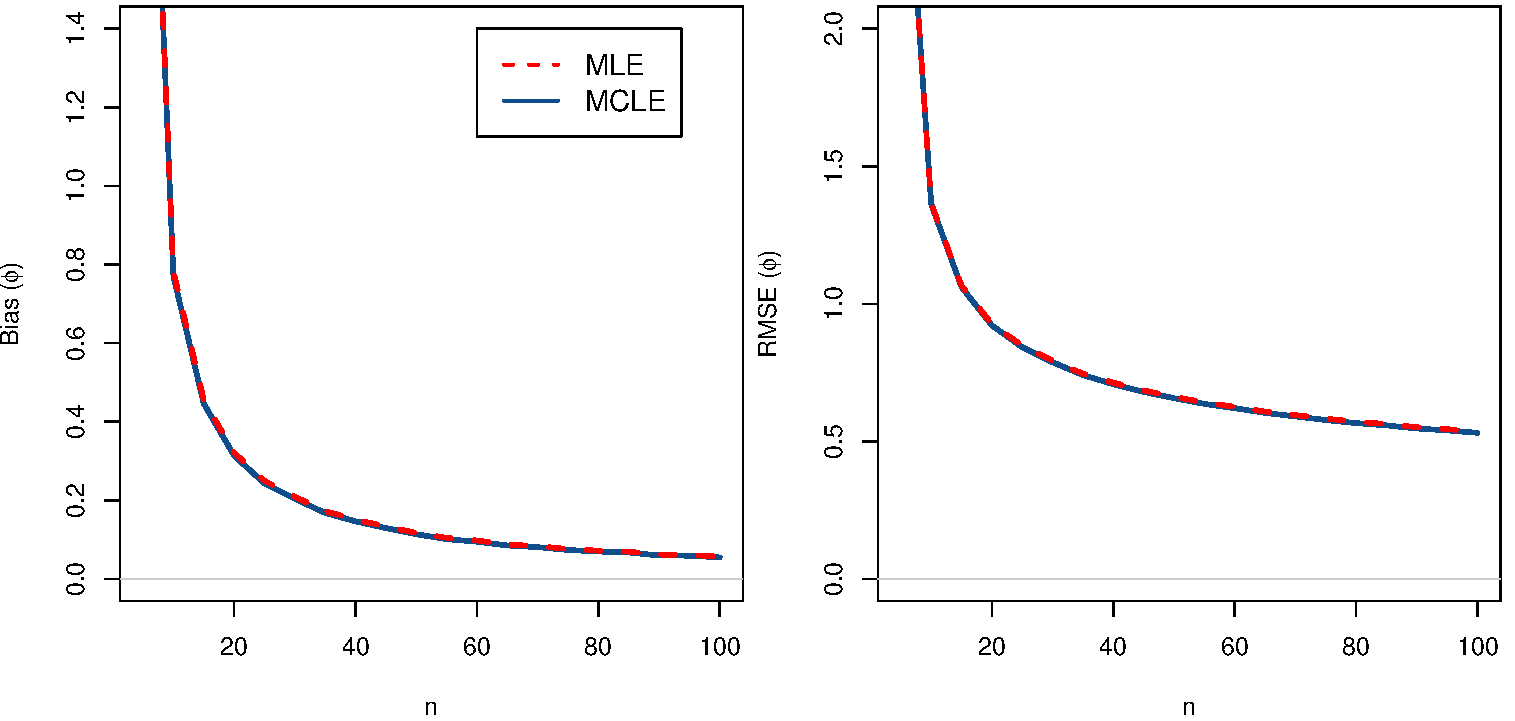
\includegraphics[scale=0.6]{biasgamma.pdf}	
\caption{Bias and RMSE for $\phi$ for samples sizes of $10,15,\ldots,100$ elements considering $\phi=2$ and $\lambda=1.5$.}\label{fg1}
\end{figure}

\noindent\textbf{Example 2:} Let $X_1$, $X_2$, $\ldots$, $X_n$ be iid random variables following a Nakagami-m distribution with PDF given by
\begin{equation*}\label{fdpnk}
f(x\,;\,\lambda,\phi)=\frac{2}{\Gamma(\phi)}\left(\frac{\phi}{\lambda} \right)^\phi t^{2\phi-1}\exp\left(-\frac{\phi}{\lambda} t^2 \right), 
\end{equation*}
for all $t>0$, where $\phi> 0.5$ and $\lambda>0$.

Once again letting $g$ as in (\ref{g}), just as in Example 1, following \cite{ramos2020bias}, as long as $X_1=\cdots=X_n$ does not hold, it follows that $\sum_{i=1}^n X_i^2 \log\left(X_i^2\right) -\frac{1}{n}\sum_{i=1}^n X_i^2\sum_{i=1}^n \log\left(X_i^2\right)\neq 0$, in which case the generalized maximum likelihood equations for $(\lambda,\phi)$ over the coordinates $(\lambda,\alpha)$ at $\alpha=2$ has as only solution
\begin{equation*}\label{vinkom}
\begin{aligned}
&\hat\lambda_n=\frac{1}{n}\sum_{i=1}^n{X_i^2} \ \ \mbox{ and } \ \
\hat\phi_n=\cfrac{\sum_{i=1}^n X_i^{2}}{\sum_{i=1}^{n}X_i^{2} \log\left(X_i^2\right) - \frac{1}{n}\sum_{i=1}^n X_i^{2} \sum_{i=1}^n \log\left(X_i^2\right)} \, \cdot
\end{aligned}
\end{equation*}

The estimator has a similar expression as that of the MMLEs of the Gamma distribution. Once again, we note these estimators are strongly consistent and asymptotically normal:

\begin{proposition}\label{proofnakagami} $\hat\phi_n$ and $\hat\lambda_n$ are strongly consistent estimators for the true parameters $\phi$ and $\lambda$, and asymptotically normal with $\sqrt{n}\left(\hat{\lambda}_n-\lambda\right)\overset{D}{\to} N\left(0,\lambda^2/\phi\right)$ and $\sqrt{n}\left(\hat{\phi}_n-\phi\right)\overset{D}{\to} N\left(0,\phi^3\psi'(\phi+1)+\phi^2\right)$.
\end{proposition}
\begin{proof} The arguments and computations involved are completely analogous to that of Proposition \ref{proofgamma}.
\end{proof}

Here, we also compare the proposed estimators with the standard MLE. In Figure \ref{fg2} we present the Bias and RMSE obtained from $100,000$ replications assuming $n=10,15,\ldots,100$ and $\phi=4$ and $\lambda=10$. We also presented only the results related to $\phi$. It can be seen from the obtained results that both estimators returned very close estimates.

\begin{figure}[!ht]
\centering
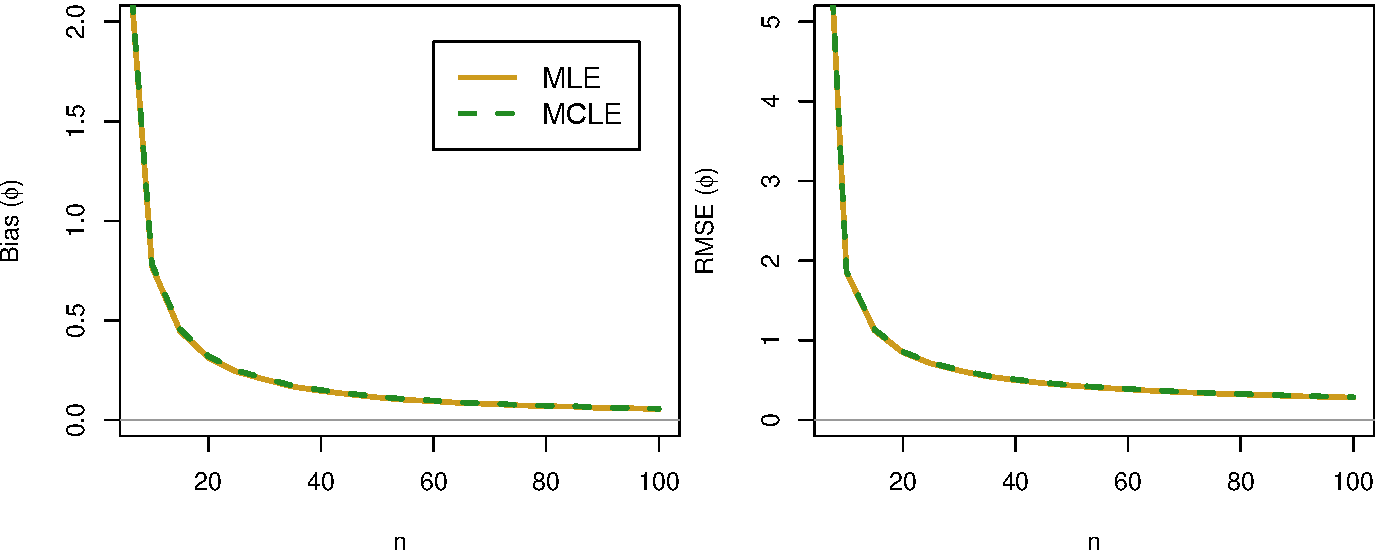
\includegraphics[scale=0.6]{biasnakagami.pdf}	
\caption{Bias and RMSE for $\phi$ for samples sizes of $10,15,\ldots,100$ elements considering $\phi=4$ and $\lambda=10$.}\label{fg2}
\end{figure}	

Note that the approach given above can be considered for other particular cases. For instance, the Wilson-Hilferty distributions are obtained when $\alpha=3$. Hence, we can obtain closed-form estimators for cited distribution as well. It is essential to mention that, in the above examples, we do not claim that the GG distribution is the unique distribution which can be used to obtain closed-form estimators for the Gamma and Nakagami distributions. Different choices for $g$ may lead to different closed-form estimators.

Now we apply the proposed approach in a generalized version of the beta distribution that will return a closed-form estimator for both parameters.
\vspace{0.3cm}

\noindent\textbf{Example 3:} Let us assume that the chosen beta distribution has the PDF given by
\begin{equation}\label{fdpbeta}
f(x\,;\,\alpha,\beta)=\frac{x^{\alpha-1}(1-x)^{\beta-1}}{\f{B}(\alpha,\beta)} \quad  0 <x<1,
\end{equation}
where $\f{B}(\alpha,\beta)=\frac{\Gamma(\alpha)\Gamma(\beta)}{\Gamma(\alpha+\beta)}$ is the beta function, $\alpha>0$, $\beta>0$.

We can apply the generalized maximum likelihood approach for this distribution by considering the function $g(x\,;\,\alpha,\beta,a,c)$ representing the generalized beta distribution,  where $\alpha>2$, $\beta>2$ given by:
\begin{equation*}g(x\,;\,\alpha,\beta,a,c)=\frac{\left(x-a\right)^{\alpha-1}\left(c-x\right)^{\beta-1}}{(c-a)^{\alpha+\beta-1}\f{B}(\alpha,\beta)}\mbox{ for all } x\in (0,1)\mbox{ and }0\leq a<x<c\leq 1.
\end{equation*}

Once, again in order to formulate the generalized maximum likelihood equations for $\bs{\theta}=(\alpha,\beta)$ over the coordinates $(a,c)$ at $(a,c)=(0,1)$ we note that
\begin{equation}\label{relations2}\on{E}_{\alpha,\beta}\left[\frac{1}{X_1}\right]=\frac{\alpha+\beta-1}{\alpha-1}\mbox{ and }\on{E}_{\alpha,\beta}\left[\frac{1}{1-X_1}\right]=\frac{\alpha+\beta-1}{\beta-1},
\end{equation}
from which it follows that
\begin{equation*}
\begin{aligned}
&\on{E}_{\alpha,\beta} \left[\frac{\partial}{\partial a}  \log g(X_1\,;\,\alpha,\beta,0,1)\right] = -(\alpha-1) \on{E}_{\alpha,\beta}\left[\frac{1}{X_1}\right] + (\alpha+\beta-1) \on{E}_{\alpha,\beta}\left[1\right]=0\mbox{ and}\\
&\on{E}_{\alpha,\beta} \left[\frac{\partial}{\partial c}  \log g(X_1\,;\,\alpha,\beta,0,1)\right] =(\beta-1) \on{E}_{\alpha,\beta}\left[\frac{1}{X_1}\right] - (\alpha+\beta-1) \on{E}_{\alpha,\beta}\left[1\right]=0.
\end{aligned}
\end{equation*}
that is, (\ref{allex}) is satisfied. Thus  the generalized likelihood equations for $\bs{\theta}=(\alpha,\beta)$ over the coordinates $(a,c)$ at $(a,c)=(0,1)$ are given by
\begin{equation*}
\begin{aligned}
&\sum_{i=1}^n \frac{\partial}{\partial a}  \log g(X_i\,;\,\alpha,\beta,0,1)=-(\alpha -1)\sum _{i=1}^{n}{\frac {1}{X_{i}}}\,+n(\alpha +\beta -1)=0,\mbox{ and }\\
&\sum_{i=1}^n \frac{\partial}{\partial c}  \log g(X_i\,;\,\alpha,\beta,0,1)=(\beta-1)\sum _{i=1}^{n}{\frac {1}{1-X_{i}}}\,-n(\alpha +\beta -1)=0.
\end{aligned}
\end{equation*}
Note that, from the harmonic-arithmetic inequality, as long as the equality $X_1=\ldots=X_n$ does not hold, we have $\sum_{i=1}^{n}\frac{1-X_i}{X_i}-\frac{n^2}{\sum_{i=1}^{n}\frac{X_i}{1-X_i}}>0$ and $\sum_{i=1}^{n}\frac{X_i}{1-X_i}-\frac{n^2}{\sum_{i=1}^{n}\frac{1-X_i}{X_i}}>0$, in which case, after some algebraic manipulations it is seem that the only solutions for the above system of linear equations are given by
%\begin{equation}\label{ecmb2}
%\hat\alpha_n=n\hat\beta_n\left(\sum_{i=1}^{n}\frac{1}{x_i}-n\right)+1,\mbox{ and }
%\end{equation}
%\begin{equation}\label{ecmb1}
%\hat\beta_n=\left(\sum_{i=1}^{n}\frac{x_i}{1-x_i}\right)\left(\sum_{i=1}^{n}\frac{x_i}{1-x_i}-n-\frac{n^2}{\sum_{i=1}^{n}\frac{1}{x_i}-n}\right)^{-1}.
%\end{equation}
%correct:
\begin{equation}\label{ecmb2}
\hat\alpha_n=\left(\sum_{i=1}^{n}\frac{1}{X_i}\right)\left(\sum_{i=1}^{n}\frac{1-X_i}{X_i}-\frac{n^2}{\sum_{i=1}^{n}\frac{X_i}{1-X_i}}\right)^{-1}.
\end{equation}
\begin{equation}\label{ecmb1}
\hat\beta_n=\left(\sum_{i=1}^{n}\frac{1}{1-X_i}\right)\left(\sum_{i=1}^{n}\frac{X_i}{1-X_i}-\frac{n^2}{\sum_{i=1}^{n}\frac{1-X_i}{X_i}}\right)^{-1}.
\end{equation}

In the following, we apply Theorem \ref{princ} prove that these estimators are consistent and asymptotically normal.

\begin{proposition} $\hat\alpha_n$ and $\hat\beta_n$ are strongly consistent estimators for the true parameters $\alpha$ and $\beta$, and asymptotically normal with $\sqrt{n}\left(\hat{\alpha}_n-\alpha\right)\overset{D}{\to} N\left(0,Q(\alpha,\beta)\right)$ and $\sqrt{n}\left(\hat{\beta}_n-\beta\right)\overset{D}{\to} N\left(0,Q(\beta,\alpha)\right)$, where
\begin{equation*}Q(y,z) = \frac{y(y - 1)^2(4yz^2 - 6z^2 - 10yz + 5y + 16z  - 10)}{(y - 2)(z - 2)(y + z - 1)}\mbox{ for all }y>2\mbox{ and }z>2.
\end{equation*}

\end{proposition}
\begin{proof} In order to apply Theorem \ref{princ}
we note $g(x\,;\,\alpha,\beta,a,c)$ can be written as \begin{equation*} g(x\,;\,\alpha,\beta,a,c)=V(x)\exp\left[\eta_1(\alpha,\beta)\log(x-a)+\eta_2(\alpha,\beta)\log(c-x)+L(\alpha,\beta,a,c)\right]
\end{equation*}
for all $x\in(0,1)$, $\alpha>2$, $\beta>2$ and $(a,c)\in\mathcal{A}_x$, with $\mathcal{A}_x$ representing the restriction $0\leq a<x<c\leq 1$, where
\begin{equation*}
\begin{aligned}V(x)=1,\ \eta_1(\alpha,\beta)=\alpha-1,\ \eta_2(\alpha,\beta)=\beta-1\mbox{ and }\\
L(\alpha,\beta,a,b)=-(\alpha+\beta-1)\log(c-a)-\log(\on{B}(\alpha,\beta)).
\end{aligned} 
\end{equation*}

In order to check condition $(A)$ of Theorem \ref{princ} note that for $a=0$ and $c=1$, following the computation of the Fisher information matrix for $g$ given in \cite{aryal2004information}, we have 
\begin{equation}
J(\alpha,\beta)=
\begin{bmatrix}
\frac {\beta }{(\alpha -1)} &  -1\\
1  & - \frac{\alpha }{(\beta -1)}
\end{bmatrix}\mbox{ and }K(\alpha,\beta)=\begin{bmatrix}
\frac {\beta(\alpha+\beta-1) }{(\alpha -2)} &   \alpha+\beta-1\\
\alpha+\beta-1  & \frac {\alpha(\alpha+\beta-1) }{(\beta -2)}
\end{bmatrix}.
\end{equation}
Thus, since $\alpha+\beta-1>0$, it is easy to see $J (\alpha,\beta)$ is invertible with
\begin{equation*}
 (J(\alpha,\beta))^{-1} = \begin{bmatrix}
\frac {\alpha(\alpha-1)}{\alpha+\beta -1} &   -\frac{(\alpha-1)(\beta-1)}{\alpha+\beta-1}\\
\frac{(\alpha-1)(\beta-1)}{\alpha+\beta-1} &  -\frac {\beta(\alpha-1)}{\alpha+\beta -1}
\end{bmatrix}.
\end{equation*}
Therefore we conclude condition $(A)$ is satisfied, and after some algebraic computations one may find that
\begin{equation}\label{compfinal2}(J(\alpha,\beta)^{-1})^T K(\alpha,\beta)J(\alpha,\beta)^{-1}=\begin{bmatrix}
Q(\alpha,\beta) &   Q_1(\alpha,\beta)\\
Q_1(\alpha,\beta) & Q(\beta,\alpha)
\end{bmatrix}.
\end{equation}
where $Q(y,z)$ is as in the proposition and $Q_1(y,z)$ is a rational function on $y$ and $z$.

Once again, item $(B)$ is straightforward to check from (\ref{relations2}). Thus, conditions $(A)$ and $(B)$ of Theorem \ref{princ} are valid, and therefore, following the same arguments as in the proof of Proposition \ref{proofgamma}, the proposition follows from the conclusion of Theorem \ref{princ} combined with (\ref{compfinal2}).
\end{proof}

Figure \ref{fg3} provides the Bias and RMSE obtained from $100,000$ replications assuming $n=10,15,\ldots,100$ and $\alpha=3$ and $\beta=2.5$. Here we considered the proposed estimator and compared with the standard MLE that does not have a closed-form expression.
\begin{figure}[!ht]
\centering
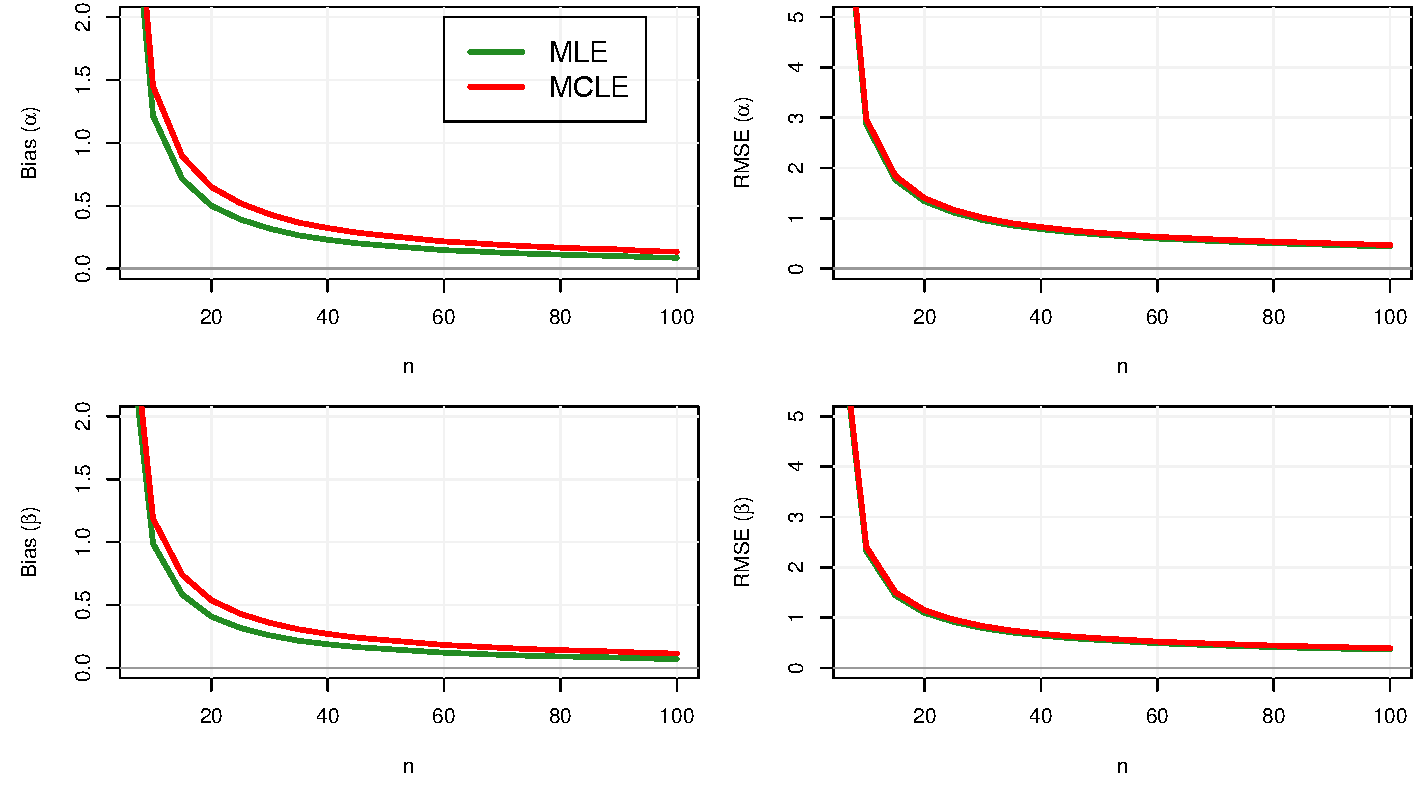
\includegraphics[scale=0.58]{biasbeta.pdf}	
\caption{Bias and RMSE for $\alpha$ and $\beta$ for samples sizes of $10,15,\ldots,100$ elements considering $\alpha=3$ and $\beta=2.5$.}\label{fg3}
\end{figure}

Unlike the Gamma and Nakagami distributions, we observed that the closed-form estimator has an additional bias. Although they are obtained from different distributions for many parameter values, they returned similar results. A major drawback of the estimators (\ref{ecmb2}) and (\ref{ecmb1}) is that the properties that ensure the consistency and asymptotic normality do not hold when the values of $\alpha$ and $\beta$ are smaller than $2$.

\noindent\textbf{Example 4:} Let us consider that $(X_1,Y_1)$, $(X_2,Y_2)$, $\ldots$, $(X_n,Y_n)$   are iid random variables (RV) following a gamma distribution with probability density function (PDF) given by:
\begin{equation}\label{fdpbigamma}
f(x, y\,;\, \beta,\alpha_1,\alpha_2) = \frac{1}{\beta^{\alpha^*_2}\Gamma(\alpha_1)\Gamma(\alpha_2)} x^{\alpha_1 - 1} (y - x)^{\alpha_2 - 1} e^{-\frac{y}{\beta}},\mbox{ where } 0 < x < y < \infty
\end{equation}
where $\phi>0$ is the shape parameter,  $\lambda>0$ is the scale parameter and $\Gamma(\alpha)=\int_{0}^{\infty}{e^{-x}x^{\alpha-1}dx}$ is the  gamma function.

We can apply the generalized maximum likelihood approach for this distribution by considering the density function $g(x,y\,;\,\beta,\alpha_1,\alpha_2,\gamma_1,\gamma_2)$ representing the generalized gamma distribution,  where $\beta$, $\alpha_1$, $\alpha_2$, $\gamma_1$ and $\gamma_2$ are positive values, given by
\begin{equation*}g(x,y\,;\,\beta,\alpha_1,\alpha_2,\gamma_1,\gamma_2) = \frac{1}{\beta^{\alpha^*_2} \Gamma(\alpha_1)\Gamma(\alpha_2)} x^{\alpha_1\gamma_1-1} \left(y^{\gamma_2} - x^{\gamma_1}\right)^{\alpha_2-1} e^{-\frac{y^{\gamma_2}}{\beta}} \left| \gamma_1\gamma_2 \right| y^{\gamma_2 - 1}
\end{equation*}

In order to formulate the generalized maximum likelihood equations for this distribution we first note that
\begin{equation*}
\begin{aligned}
\on{E}_{\bs{\theta}}\left[\log^2 Z_1\right] = & \phi_1(\alpha_1) + \left[\phi(\alpha_1) + \log \beta\right]^2, \\
\on{E}_{\bs{\theta}}\left[Z_1 \log^2 Z_1\right] = & \alpha_1\beta\left\{ \phi_1(\alpha_1 + 1) + \left[\phi(\alpha_1 + 1) + \log \beta\right]^2\right\}, \\
\on{E}_{\bs{\theta}}\left[Z_2 \log Z_1\right] =& \alpha_1\beta \left[\phi(\alpha_1 + 1) + \log \beta\right] + \alpha_2\beta \left[\phi(\alpha_1) + \log \beta\right], \\
\on{E}_{\bs{\theta}}\left[Z_2^2 \log Z_2
\right] = & (\alpha_1 + \alpha_2 + 1)(\alpha_1 + \alpha_2)\beta^2
\left[\phi(\alpha_1 + \alpha_2 + 2) + \log \beta\right], \\
\on{E}_{\bs{\theta}}\left[Z_2 \log^2 Z_2\right] = &(\alpha_1 + \alpha_2)\beta
\left\{\phi_1(\alpha_1 + \alpha_2 + 1) + \left[\phi(\alpha_1 + \alpha_2 + 1) + \log\beta\right]^2
\right\}, \\
\on{E}_{\bs{\theta}}\left[Z_2^2 \log^2
Z_2\right] = & (\alpha_1 + \alpha_2 + 1)(\alpha_1 + \alpha_2)\beta^2
\left\{\phi_1(\alpha_1 + \alpha_2 + 2) + \left[\phi(\alpha_1 + \alpha_2 + 2) + \log\beta\right]^2
\right\},
\end{aligned}
\end{equation*}

from which it follows that\begin{align*}
\on{E}_{\bs{\theta}} \left[\frac{\partial}{\partial \beta}  \log g(X_1,Y_1\,;\,\bs{\theta},1,1)\right] &= -\frac{(\alpha_1 + \alpha_2)}{\beta} + \frac{1}{\beta^2} \on{E}_{\bs{\theta}}[Y_1] = 0, \\
\on{E}_{\bs{\theta}} \left[\frac{\partial}{\partial \gamma_1}  \log g(X_1,Y_1\,;\,\bs{\theta},1,1)\right] &= \alpha_1 \on{E}_{\bs{\theta}}[\log X_1] - (\alpha_2 - 1) \on{E}_{\bs{\theta}}\left[\frac{X_1 \log X_1}{Y_1 - X_1}\right] + 1 = 0, \\
\on{E}_{\bs{\theta}} \left[\frac{\partial}{\partial \gamma_2}  \log g(X_1,Y_1\,;\,\bs{\theta},1,1)\right] &= (\alpha_2 - 1) \on{E}_{\bs{\theta}}\left[\frac{Y_1 \log Y_1}{Y_1 - X_1}\right] - \frac{1}{\beta} \on{E}_{\bs{\theta}}\left[Y_1 \log Y_1\right] + 1 + \on{E}_{\bs{\theta}}\left[\log Y_1\right]=0,
\end{align*}
that is, (\ref{allex}) is satisfied. Thus, the generalized likelihood equations for $\bs{\theta}=(\beta,\alpha_1,\alpha_2)$ over the coordinates $(\gamma_1,\gamma_2)$ at $(\gamma_1,\gamma_2)=(1,1)$ are given by
\begin{align*}
\frac{\partial}{\partial \beta}  \log g(x_j,y_j\,;\,\bs{\theta},1,1) &= -\frac{n (\alpha_1 + \alpha_2)}{\beta} + \frac{1}{\beta^2} \sum_{j=1}^{n} y_j = 0, \\
\frac{\partial}{\partial \gamma_1}  \log g(x_j,y_j\,;\,\bs{\theta},1,1) &= \alpha_1 \sum_{j=1}^{n} \log x_j - (\alpha_2 - 1) \sum_{j=1}^{n} \frac{x_j \log x_1}{y_j - x_j} + n = 0, \\
\frac{\partial}{\partial \gamma_2}  \log g(x_j,y_j\,;\,\bs{\theta},1,1) &= (\alpha_2 - 1) \sum_{j=1}^{n} \frac{y_j \log y_j}{y_j - x_j} - \frac{1}{\beta} \sum_{j=1}^{n} y_j \log y_j + n + \sum_{j=1}^{n} \log y_j = 0
\end{align*}
Following \cite{louzada2019note}, as $D\neq 0$, a direct computation shows the generalized likelihood equations above has as only solution
\begin{align*}
\hat{\alpha}_2 = -\frac{D}{C}, \
\hat{\alpha}_1 = \frac{1}{\sum_{j=1}^{n} \log x_j} \left[ (\hat{\alpha}_2 - 1) \sum_{j=1}^{n} \frac{x_j \log x_j}{y_j - x_j} - n \right], \
\hat{\beta} = \frac{\sum_{j=1}^{n} y_j}{n (\hat{\alpha}_1 + \hat{\alpha}_2)}.
\end{align*}

We now apply Theorem \ref{princ} to prove that the obtained estimators are consistent and asymptotically normal.

\begin{proposition}\label{proofgamma} $\hat\phi_n$ and $\hat\lambda_n$ are strongly consistent estimators for the true parameters $\phi$ and $\lambda$, and asymptotically normal with $\sqrt{n}\left(\hat{\lambda}_n-\lambda\right)\overset{D}{\to} N\left(0,\lambda^2/\phi\right)$ and $\sqrt{n}\left(\hat{\phi}_n-\phi\right)\overset{D}{\to} N\left(0,\phi^3\psi'(\phi+1)+\phi^2\right)$.
\end{proposition}
\begin{proof}In order to apply Theorem \ref{princ}
 we note $g(x\,;\,\lambda,\phi,\alpha)$ can be rewritten as
 \begin{equation*}
 \begin{aligned}
 g(x\,;\,\lambda,\phi,\alpha)=\frac{\alpha}{\Gamma(\phi)}\left(\frac{\phi}{\lambda} \right)^\phi x^{\alpha\phi-1}\exp\left(-\frac{\phi}{\lambda} x^\alpha \right)=\\
 V(x)\exp\left(\eta_1(\lambda,\phi)T_1(x,\alpha)+\eta_2(\lambda,\phi)T_2(x,\alpha)+L(\lambda,\phi,\alpha)\right)
 \end{aligned}
 \end{equation*}
for all $x>0$, $\lambda>0$, $\theta>0$ and $\alpha>0$, where
\begin{equation*}
\begin{aligned}V(x)=\frac{1}{x},\ \eta_1(\lambda,\phi)=\phi,\ \eta_2(\lambda,\phi)=-\frac{\phi}{\lambda}\\
T_1(x,\alpha)=\alpha\log(x),\ T_2(x,\alpha) = x^{\alpha}\mbox{ and }\\
L(\lambda,\phi,\alpha)=\log\left(\alpha\right)-\log\left(\Gamma(\phi)\right)+\phi\log\left(\frac{\phi}{\lambda}\right).
\end{aligned}
\end{equation*}

To check condition $(A)$ of Theorem \ref{princ} note that, for $\alpha=1$ and using reparametrization over the Fisher information matrix from the GG distribution available in \cite{1970-Hager} it follows that the Fisher information matrix under our parametrization satisfy
\begin{equation}\label{mfishergg}
I(\lambda,\phi,\alpha_0)=
\begin{bmatrix}
\dfrac{\phi}{\lambda^2}  & 0 & \frac{\phi \log\left(\frac{\phi}{\lambda}\right) - \phi\psi(\phi) - 1}{\lambda} \\
 0 & \frac{\phi\psi'(\phi) - 1}{\phi}  & \frac{1}{\phi}  \\
\frac{\phi \log\left(\frac{\phi}{\lambda}\right) - \phi\psi(\phi) - 1}{\lambda} &  \frac{1}{\phi} & I_{3,3}(\lambda,\phi)
\end{bmatrix},
\end{equation}
for $\alpha_0=1$, where
\begin{equation*}
I_{3,3}(\lambda,\phi) = \log\left(\frac{\phi}{\lambda}\right)\left(\phi\log\left(\frac{\phi}{\lambda}\right) -2\phi\psi(\phi)-2\right) + \phi\psi'(\phi) + 2\psi(\phi) + \phi\psi(\phi)^2 + 1.
\end{equation*}
Therefore since, as discussed earlier, $J(\lambda,\phi)$ and $K(\lambda,\phi)$ can be computed as submatrices of $I(\lambda,\phi,\alpha_0)$, we have
\begin{equation}\label{mfishergg2}
J(\lambda,\phi)=
\begin{bmatrix}
 \dfrac{\phi}{\lambda^2}  & \frac{\phi \log\left(\frac{\phi}{\lambda}\right) - \phi\psi(\phi) - 1}{\lambda}\\
 0 &  \frac{1}{\phi}
\end{bmatrix}\mbox{ and } 
K(\lambda,\phi)=\begin{bmatrix}
 \dfrac{\phi}{\lambda^2}  & \frac{\phi \log\left(\frac{\phi}{\lambda}\right) - \phi\psi(\phi) - 1}{\lambda}\\
 \frac{\phi \log\left(\frac{\phi}{\lambda}\right) - \phi\psi(\phi) - 1}{\lambda} &  I_{3,3}(\lambda,\phi)
\end{bmatrix},
\end{equation}
and thus, since $\det(J(\lambda,\phi))=\frac{1}{\lambda^2}\neq 0$, it follows that $J(\lambda,\phi)$ is invertible for all $\phi>0$ and $\lambda>0$ with
\begin{equation*}
J(\lambda,\phi)^{-1}=\begin{bmatrix}
\frac{\lambda^2}{\phi}   & -\lambda \left(\phi \log\left(\frac{\phi}{\lambda}\right) - \phi\psi(\phi) - 1\right)\\
0 &  \phi
\end{bmatrix},
\end{equation*}
that is, condition $(A)$ is verified. Additionally, after some algebraic computations, one can verify that
\begin{equation}\label{compfinal} (J(\lambda,\phi)^{-1})^T K(\lambda,\phi)J(\lambda,\phi)^{-1}= \begin{bmatrix}
\frac{\lambda^2}{\phi}   & 0\\
0 &  \phi^3 \psi'(\phi+1) + \phi^2
\end{bmatrix}.
\end{equation}

Item $(B)$ is straightforward to check from (\ref{princ}). Thus conditions $(A)$ and $(B)$ of Theorem \ref{princ} are valid and therefore, from Theorem \ref{princ}, we conclude there exist $\bs{\hat{\theta}}_n(\bs{x})=(\hat{\theta}_{1n}(\bs{x}),\cdots,\hat{\theta}_{sn}(\bs{x}))$ measurable in $\bs{x}\in \mathcal{X}^n$ satisfying items $I)$ to $III)$ of Theorem \ref{princ}.

 Now, since the equation $X_1=\cdots=X_n$ has probability zero of ocurring for $n\geq 2$, it follows that $(\hat\lambda_n,\hat\phi_n)$ as given in (\ref{verogg21}) is, with probability one, the only solution of the generalized maximum likelihood equations for $n\geq 2$.
This fact combined with item $I)$ of Theorem \ref{princ} implies that $\bs{\hat{\theta}}_n(\bs{X})\overset{a.s.}{\to} (\hat\lambda_n,\hat\phi_n)$. Thus the proposition follows from items $II)$ and $III)$ of Theorem \ref{princ}  combined with (\ref{compfinal}).
\end{proof}

Note that the MLE of $\phi$ differs from the obtained using our approach, which leads to a closed-form expression. Figure \ref{fg1} presents the Bias and root of the mean square error (RMSE) obtained from $100,000$ replications assuming $n=10,15,\ldots,100$ and $\phi=2$ and $\lambda=1.5$. We presented only the results related to $\phi$, since the estimator of $\lambda$ is the same using both approaches. It can be seen from the obtained results that both estimators' results in similar (although not the same) results.


%\noindent\textbf{Example 4:} Let us assume that the chosen Windley distribution has the PDF given by
%\begin{equation}\label{fdpbeta}
%f(x\,;\,\lambda,\phi)=\frac{\lambda^{\phi+1}}{(\lambda+\phi)\Gamma(\phi)}x^{\phi-1}(1+x)\exp(-\lambda x) \quad  x>0,
%\end{equation}
%where $\lambda>0$ and  $\phi>0$.

%We can apply the generalized maximum likelihood approach for this distribution by considering the function $g(x\,;\,\lambda,\phi,\alpha)$,  where $\lambda>0$, $\phi>0$ and $\alpha>0$, given by:
%\begin{equation*}g(x\,;\,\lambda,\phi,\alpha)=\frac{\alpha\lambda^{\alpha\phi+1}}{(\lambda+\phi)\Gamma(\phi)}x^{\phi-1}(1+x)\exp(-\lambda x^\alpha) \mbox{ for all } x>0
%\end{equation*}

%Note $f(x\,;\, \lambda,\phi)=g(x\,;\,\lambda,\phi,1)$. Thus we can consider the generalized likelihood equations for $g$ over $\alpha=1$ for $s=1$ and $r=1$, which are given by
%\begin{equation*}
%\begin{aligned}
%&\sum_{i=1}^n \frac{\partial}{\partial \alpha}  \log g(X_i\,;\,\alpha,\beta,0,1)=-(\alpha -1)\sum _{i=1}^{n}{\frac {1}{X_{i}}}\,+n(\alpha +\beta -1)=0,\mbox{ and }\\
%&\sum_{i=1}^n \frac{\partial}{\partial c}  \log g(X_i\,;\,\alpha,\beta,0,1)=(\beta-1)\sum _{i=1}^{n}{\frac {1}{1-X_{i}}}\,-n(\alpha +\beta -1)=0.
%\end{aligned}
%\end{equation*}
%Note that, from the harmonic-arithmetic inequality, as long as the equality $X_1=\cdots=X_n$ does not hold, we have $\sum_{i=1}^{n}\frac{1-X_i}{X_i}-\frac{n^2}{\sum_{i=1}^{n}\frac{X_i}{1-X_i}}>0$ and $\sum_{i=1}^{n}\frac{X_i}{1-X_i}-\frac{n^2}{\sum_{i=1}^{n}\frac{1-X_i}{X_i}}>0$, in which case, after some algebraic manipulations it is seem that the only solutions for the above system of linear equations are given by
%\begin{equation}\label{ecmb2}
%\hat\alpha_n=n\hat\beta_n\left(\sum_{i=1}^{n}\frac{1}{x_i}-n\right)+1,\mbox{ and }
%\end{equation}
%\begin{equation}\label{ecmb1}
%\hat\beta_n=\left(\sum_{i=1}^{n}\frac{x_i}{1-x_i}\right)\left(\sum_{i=1}^{n}\frac{x_i}{1-x_i}-n-\frac{n^2}{\sum_{i=1}^{n}\frac{1}{x_i}-n}\right)^{-1}.
%\end{equation}
%correct:
%\begin{equation}\label{ecmb2}
%\hat\alpha_n=\left(\sum_{i=1}^{n}\frac{1}{X_i}\right)\left(\sum_{i=1}^{n}\frac{1-X_i}{X_i}-\frac{n^2}{\sum_{i=1}^{n}\frac{X_i}{1-X_i}}\right)^{-1}.
%\end{equation}
%\begin{equation}\label{ecmb1}
%\hat\beta_n=\left(\sum_{i=1}^{n}\frac{1}{1-X_i}\right)\left(\sum_{i=1}^{n}\frac{X_i}{1-X_i}-\frac{n^2}{\sum_{i=1}^{n}\frac{1-X_i}{X_i}}\right)^{-1}.
%\end{equation}

%In the following, we prove that these estimators are consistent and asymptotically normal.

%\begin{proposition} $\hat\alpha_n$ and $\hat\beta_n$ are strongly consistent estimators for the true parameters $\alpha$ and $\beta$, and asymptotically normal with $\sqrt{n}\left(\hat{\alpha}_n-\alpha\right)\overset{D}{\to} N\left(0,Q(\alpha,\beta)\right)$ and $\sqrt{n}\left(\hat{\beta}_n-\beta\right)\overset{D}{\to} N\left(0,Q(\beta,\alpha)\right)$, where
%\begin{equation*}Q(y,z) = \frac{y(y - 1)^2(4yz^2 - 6z^2 - 10yz + 5y + 16z  - 10)}{(y - 2)(z - 2)(y + z - 1)}\mbox{ for all }y>2\mbox{ and }z>2.
%\end{equation*}

%\end{proposition}
%\begin{proof} In order to apply Theorem \ref{princ}
% we note $g(x\,;\,\alpha,\beta,a_0,c_0)$ can be written as \begin{equation*} g(x\,;\,\alpha,\beta,a_0,c_0)=V(x)\exp\left[\eta_1(\alpha,\beta)\log(x-a_0)+\eta_2(\alpha,\beta)\log(c_0-x)+L(\alpha,\beta,a_0,c_0)\right]
% \end{equation*}
%for all $x\in\left]a_0,c_0\right[$, $\alpha>2$, $\beta>2$ and $a_0<c_0$, where
%\begin{equation*}
%\begin{aligned}V(x)=1,\ \eta_1(\alpha,\beta)=\alpha-1,\ \eta_2(\alpha,\beta)=\beta-1\mbox{ and }\\
%L(\alpha,\beta,a_0,b_0)=-(\alpha+\beta-1)\log(c_0-a_0)-\log(\on{B}(\alpha,\beta)).
%\end{aligned} 
%\end{equation*}

%In order to check condition $(A)$ of Theorem \ref{princ} we note that from the discussion above, the generalized likelihood equations has $(\hat{\alpha}_n,\hat{\beta}_n)$ as its only solution unless $X_1=X_2=\cdots=X_n$, which has probability zero of occurring if $n\geq 2$.
%In order to check condition $(B)$ of Theorem \ref{princ} note that for $a=a_0$ and $c=c_0$, following the computations of \cite{aryal2004information}, we have 
%\begin{equation}
%J(\alpha,\beta)=
%\begin{bmatrix}
%\frac {\beta }{(\alpha -1)} &  -1\\
%1  & - \frac{\alpha }{(\beta -1)}
%\end{bmatrix}\mbox{ and }K(\alpha,\beta)=\begin{bmatrix}
%\frac {\beta(\alpha+\beta-1) }{(\alpha -2)} &   \alpha+\beta-1\\
%\alpha+\beta-1  & \frac {\alpha(\alpha+\beta-1) }{(\beta -2)}
%\end{bmatrix}.
%\end{equation}
%Thus, since $\alpha+\beta-1>0$, it is easy to see $J (\alpha,\beta)$ is invertible with
%\begin{equation*}
%(J(\alpha,\beta))^{-1} = \begin{bmatrix}
%\frac {\alpha(\alpha-1)}{\alpha+\beta -1} &  % -\frac{(\alpha-1)(\beta-1)}{\alpha+\beta-1}\\
% \frac{(\alpha-1)(\beta-1)}{\alpha+\beta-1} &  -\frac {\beta(\alpha-1)}{\alpha+\beta -1}
%\end{bmatrix}.
%\end{equation*}
%Therefore we conclude condition $(B)$ is satisfied, and after some algebraic computations one may find that
%\begin{equation}\label{compfinal2}(J(\alpha,\beta)^{-1})^T K(\alpha,\beta)J(\alpha,\beta)^{-1}=\begin{bmatrix}
%  Q(\alpha,\beta) &   Q_1(\alpha,\beta)\\
% Q_1(\alpha,\beta) & Q(\beta,\alpha)
%\end{bmatrix}.
%\end{equation}
%where $Q(y,z)$ is as in the proposition and $Q_1(y,z)$ is a rational function on $y$ and $z$. Condition $(C)$ of Theorem \ref{princ} follows analogously as in the proof of Proposition \ref{proofgamma}, by noting the relations:
%\begin{equation*}\on{E}_{\alpha,\beta}\left[\frac{1}{X_1}\right]=\frac{\alpha+\beta-1}{\alpha-1}\mbox{ and }\on{E}_{\alpha,\beta}\left[\frac{1}{1-X_1}\right]=\frac{\alpha+\beta-1}{\beta-1}.
%\end{equation*}
%Finally, condition $(D)$ of Theorem \ref{princ} follows by noting that $\pi:(2,\infty)^2\to (1,\infty)^2$ given by $\pi(\alpha,\beta)=\left(\eta_1(\alpha,\beta),\eta_2(\alpha,\beta)\right)=(\alpha-1,\beta-1)$ is a diffeomorphism. Thus, we verified conditions $(A)$ to $(D)$ of Theorem \ref{princ}, and therefore the proposition follows from the conclusion of Theorem \ref{princ} combined with (\ref{compfinal2}).
%\end{proof}

%Figure \ref{fg3} provides the Bias and RMSE obtained from $100,000$ replications assuming $n=10,15,\ldots,100$ and $\alpha=3$ and $\beta=2.5$. Here we considered the proposed estimator and compared with the standard MLE that does not have a closed-form expression.
%\begin{figure}[!ht]
%\centering
%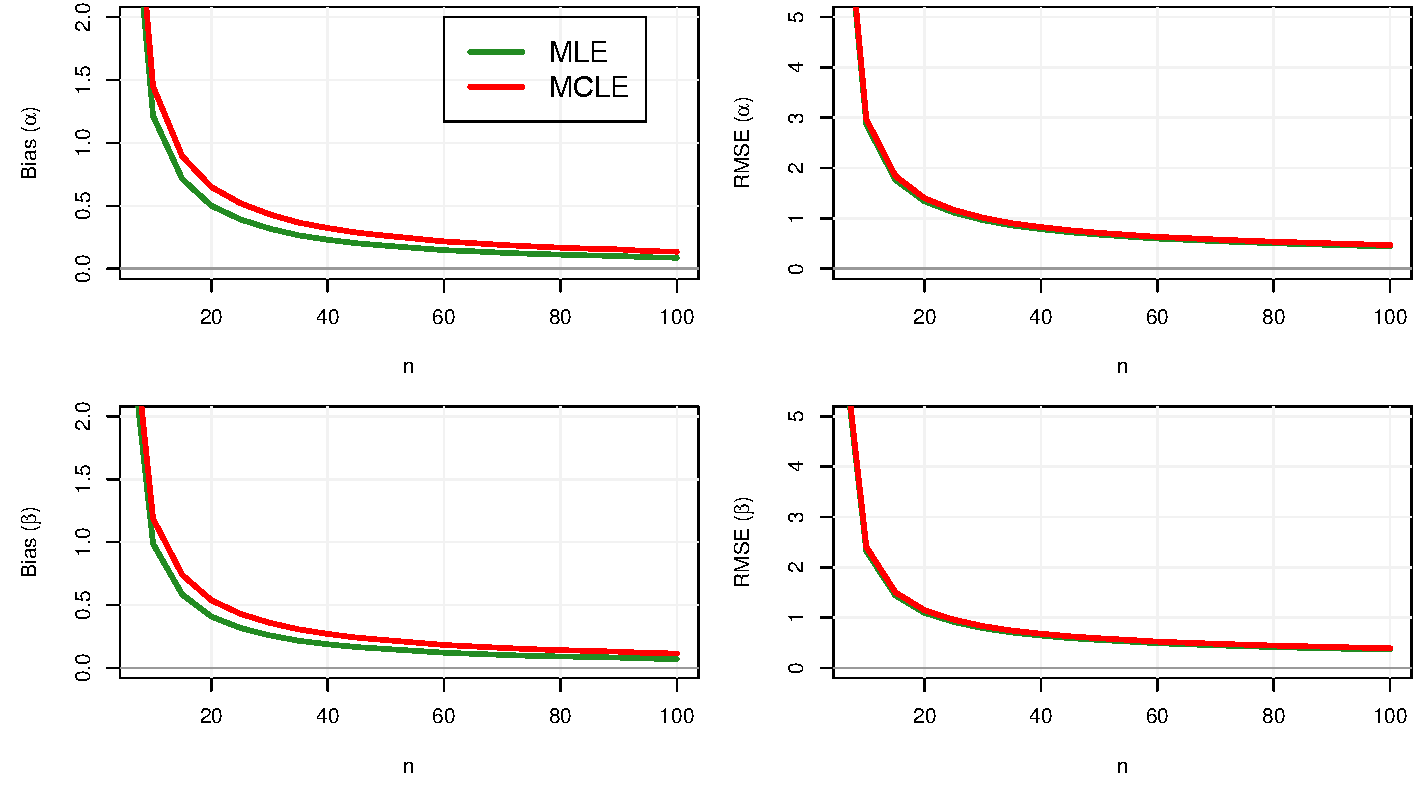
\includegraphics[scale=0.58]{biasbeta.pdf}	
%\caption{Bias and RMSE for $\alpha$ and $\beta$ for samples sizes of $10,15,\ldots,100$ elements considering $\alpha=3$ and $\beta=2.5$.}\label{fg3}
%\end{figure}

%Unlike the Gamma and Nakagami distributions, we observed that the closed-form estimator has an additional bias. Although they are obtained from different distributions for many parameter values, they returned similar results. A major drawback of the estimators (\ref{ecmb2}) and (\ref{ecmb1}) is that the properties that ensure the consistency and asymptotic normality do not hold when the values of $\alpha$ and $\beta$ are smaller than $2$.



\section{Final Remarks}

We have shown that the proposed generalized version of the maximum likelihood estimators provides a vital alternative to achieve closed-form expressions when the standard MLE approach fails. The proposed approach can also be used with discrete distributions, the results remain valid, and the obtained estimators are still consistent, invariant, and is asymptotic normally distributed. Due to the likelihood function's flexibility, additional complexity can be included in the distribution and the inferential procedure such as censoring, long-term survival, covariates, and random effects.

The introduced method can, in special, be obtained from the use of generalized versions of the baseline distribution. Hence, it provides another important motivation for applying many new distributions that have been introduced in the past few decades. Additionally, as the estimators are not unique and depend on the generalized distribution, comparisons between the different estimators are encouraged to find the one with better performance in terms of a specific metric. 

As shown in Examples 1 and 2, the estimators' behaviors in terms of Bias and RMSE are similar to those obtained under the MLE for the Gamma and Nakagami distributions. Therefore, corrective bias approaches can also be used to remove the bias of the generalized estimators. For the Beta distribution, the comparison showed different behavior for the proposed estimators. We observed that for specific small values of the parameters, the results might not be consistent. This example illustrates what happens in situations where, for some parameter values, the Fisher information of the generalized distribution has singularity problems.


\section*{Disclosure statement}

No potential conflict of interest was reported by the author(s).


\section*{Acknowledgements}

 Eduardo Ramos acknowledges financial support from S\~ao Paulo State Research Foundation (FAPESP Proc. 2019/27636-9). This work has benefited from FAPESP  grant 1/22308-2. Francisco Rodrigues acknowledges financial support from CNPq (grant number 309266/2019-0). Francisco Louzada is supported by the Brazilian agencies CNPq (grant number
301976/2017-1) and FAPESP (grant number 2013/07375-0).

\section*{Appendix}
\begin{appendix}


In order to prove Theorem \ref{princ} we shall need the tecnical lemma that follows.

In the following, given $\bs{x}\in \R^m$ we let $\left\|\bs{x}\right\|_2=\sqrt{\sum_{i=1}^m x_i^2}$ and given a matrix $A\in M_m(\R)$ we let $\left\|A\right\|_2$ denote the usual spectral norm defined by $\left\|A\right\|_2=\sup_{\left\|x\right\|=1}\left\|Ax^T\right\|_2$. Moreover, given a differentiable function $F:\Theta\to \mathbb{R}^m$, for $\Theta\subset \mathbb{R}^m$ open, we denote $\frac{\partial}{\partial \theta_j} F(\bs{\theta})=\left(\frac{\partial}{\partial \theta_j} F_1 (\bs{\theta}),\cdots,  \frac{\partial}{\partial \theta_j} F_n (\bs{\theta})\right)$, and we denote
 by $\frac{\partial}{\partial \bs{\theta}} F(\bs{\theta})$ the Jacobian of $F$ at $\bs{\theta}\in \Theta$, that is, $\frac{\partial}{\partial \bs{\theta}} F(\bs{\theta})=\left(\frac{\partial}{\partial \theta_j} F_i (\bs{\theta})\right)\in M_m(\mathbb{R})$ for all $\bs{\theta}\in \Theta$.
 
\begin{lemma}\label{clemma} Let $\Theta\subset \mathbb{R}^m$ be open, let $F:\Theta\to \mathbb{R}^m$ be $C^1$, let $J\in  M_m(\mathbb{R})$ be invertible, denote $\lambda = \frac{1}{2} \left\|J^{-1}\right\|_2^{-1}$ and $r=\frac{1}{\lambda}\left\|F(\theta_0)\right\|_2$, and suppose that:
\begin{equation*}
\begin{aligned}\bar{B}(\bs{\theta}_0,r)\subset \Theta\mbox{ and }
\left\|\frac{\partial}{\partial \bs{\theta}} F(\bs{\theta})-J\right\|_2\leq \lambda \mbox{ for all }\theta\in \bar{B}(\bs{\theta}_0,r),
\end{aligned}
\end{equation*}
Then there exist $\bs{\theta}^*\in \bar{B}(\bs{\theta}_0,r)$ such that $F(\bs{\theta}^*)=0$.
\end{lemma}

 \begin{proof} The proof shall follow from a simple application of the Browder Fixed Point Theorem.

Letting $L:\bar{B}(\bs{\theta}_0,r)\to \mathbb{R}^m$ be defined by
$L(\bs{\theta})=\bs{\theta}-J^{-1} \frac{\partial}{\partial \bs{\theta}} F(\bs{\theta})$ for all $\bar{B}(\bs{\theta}_0,r)$
we shall prove that $L(\bar{B}(\bs{\theta}_0,r))\subset \bar{B}(\bs{\theta}_0,r)$. Indeed, from the chain rule it follows that $L$ is differentiable in $\bar{B}(\bs{\theta}_0,r)$ with
\begin{equation*}
L'(\bs{\theta})=I-J^{-1} \frac{\partial}{\partial \bs{\theta}}F(\bs{\theta})=J^{-1}\left(J-\frac{\partial}{\partial \bs{\theta}} F(\bs{\theta})\right)\mbox{ for all }\bs{\theta}\in \Theta.
\end{equation*}
Thus, for all $\bs{\theta}\in \bar{B}(\bs{\theta}_0,r)$ we have
\begin{equation*}
\begin{aligned}
\label{peq1}
\left\|\frac{\partial}{\partial \bs{\theta}} L(\bs{\theta})\right\|_2=\left\|J^{-1}\left(J-\frac{\partial}{\partial \bs{\theta}} F(\bs{\theta})\right)\right\|_2\leq \left\|J^{-1}\right\|_2\left\|J-\frac{\partial}{\partial \bs{\theta}} F(\bs{\theta})\right\|_2\leq \frac{1}{2},
\end{aligned}
\end{equation*}
and thus from the mean value inequality we have
\begin{equation}\label{ineq3}
\left\|L(\bs{\theta})-L(\bs{\theta}_0)\right\|_2\leq \frac{1}{2} \left\|\theta-\theta_0\right\|_2\leq \frac{r}{2}\mbox{ for all }\bs{\theta}\in \bar{B}(\bs{\theta}_0,r).
\end{equation}
Moreover, note that
\begin{equation}\label{peq2}\left\|L(\bs{\theta}_0)-\bs{\theta}_0\right\|_2=\left\|J^{-1}F(\bs{\theta}_0)\right\|_2\leq \left\|J^{-1}\right\|_2\left\|F(\bs{\theta}_0)\right\|_2 =\frac{1}{2\lambda}\left\|F(\bs{\theta}_0)\right\|_2=\frac{r}{2}
\end{equation}
Thus, given $\bs{\theta}\in \bar{B}(\bs{\theta}_0,r)$ from inequalities (\ref{ineq3}) and  (\ref{peq2}) and the triangle inequality we have
\begin{equation*}
\begin{aligned}
\left\|L(\bs{\theta})-\bs{\theta}_0\right\|_2\leq \left\|L(\bs{\theta})-L(\bs{\theta}_0)\right\|_2+\left\|L(\bs{\theta}_0)-\bs{\theta}_0\right\|_2\leq \frac{r}{2}+\frac{r}{2}= r,
\end{aligned}
\end{equation*}
that is, $L(\bs{\theta})\in \bar{B}(\bs{\theta}_0,r)$ for all $\theta\in \bar{B}(\theta_0,r)$, which proves that $L(\bar{B}(\bs{\theta}_0,r)\subset \bar{B}(\bs{\theta}_0,r)$. Thus, since $L:\bar{B}(\bs{\theta}_0,r)\to \bar{B}( \bs{\theta}_0,r)$ is continuous, from the Browder Fixed Point Theorem we conclude $L$ has at least one fixed point $\bs{\theta}^*$ in $\bar{B}(\bs{\theta}_0,r)$, and thus
\begin{equation*}L(\bs{\theta}^*)=\bs{\theta}^*\Rightarrow J^{-1}F(\bs{\theta}^*)=0\Rightarrow F(\bs{\theta}^*)=0
\end{equation*}
which concludes the proof.
\end{proof}

%From this result it is easy to prove the following.

%\begin{lemma}\label{clemma} Let $\Theta\subset \mathbb{R}^m$ be open, let $F_i:\Theta\to \mathbb{R}^m$ be differentiable for all $i\in \mathbb{N}$, let $\bs{\theta}_0\in \Theta$ and suppose that
%\begin{equation*}\lim_{n\to \infty} F_n(\bs{\theta}_0)=0\mbox{ and }\lim_{n\to \infty}F_n'(\bs{\theta})=G(\bs{\theta})\mbox{ uniformly on }\Theta,
%\end{equation*}
%where $G:\Theta\to M_m(\mathbb{R})$ is continuous at $\bs{\theta}_0$ and $G(\bs{\theta}_0)$ is invertible. Then there exists $N>0$ and a sequence $\{\bs{\theta}_n\}_{n\geq N}$ in $\Theta$ such that
%\begin{equation}\label{lcond}\lim_{n\to \infty} \bs{\theta}_n = \bs{\theta}_0 \mbox{ and }F_n(\bs{\theta}_n)=0
%\mbox{ for all } n\geq N,
%\end{equation}
%\end{lemma}

%\begin{proof} Let $\lambda=2\left\|G(\bs{\theta}_0)^{-1}\right\|^{-1}$ and $\epsilon_n=\frac{1}{\lambda}\left\|F_n(\bs{\theta}_0)\right\|$. Since due to hypothesis $\Theta$ is open and $G$ is continuous at $\bs{\theta}_0$, there exist $\delta>0$ such that \begin{equation}B(\bs{\theta}_0,\delta)\subset \Theta\mbox{ and }\label{leq1}\left\|G(\bs{\theta})-G(\bs{\theta}_0)\right\|< \frac{\lambda}{2}\mbox{ for all }\bs{\theta}\in B(\bs{\theta}_0,\delta).
%\end{equation}
%and also due to the hypothesis there must exist $N>0$ such that $n\geq N$ implies in
%\begin{equation}\label{leq2}
%\left\|F_n(\bs{\theta}_0)\right\|< \delta \lambda\mbox{ and }\left\| F_n'(\bs{\theta})-G(\bs{\theta})\right\|< \frac{\lambda}{2}\mbox{ for all }\bs{\theta}\in \Theta.
%\end{equation}
%From the first inequality in (\ref{leq2}) it follows that $\epsilon_n< \delta$ for all $n\geq N$, which implies in $\bar{B}(\bs{\theta}_0,\epsilon_n)\subset B(\bs{\theta}_0,\delta)\subset \Theta$ for all  $n\geq N$.
 
%Now, the inequality in (\ref{leq1}) combined with the second inequality in (\ref{leq2})  the triangle inequality and $\bar{B}(\bs{\theta}_0,\epsilon_n)\subset \bar{B}(\bs{\theta}_0,\delta)$ implies that
%\begin{equation}\label{leq3} \left\|F_n'(\bs{\theta})-G(\bs{\theta}_0)\right\|< \lambda \mbox{ for all }\bs{\theta}\in B(\bs{\theta}_0,\epsilon_n)\mbox{ and }n\geq N.
%\end{equation}
%Thus from Lemma (\ref{clemma}) $F_n$ has a zero $\bs{\theta}_n$ in $\bar{B}(\bs{\theta}_0,\epsilon_n)$, for all $n \geq N$ but since by hypothesis $\lim_{n\to \infty} \epsilon_n =\lim_{n\to \infty}\frac{1}{\lambda} F_n(\bs{\theta}_0)=0$ it follows that $\lim_{n\to \infty} \bs{\theta}_n = \bs{\theta}_0$, and thus the Lemma follows.
%\end{proof}

Additionally we shall need the following lemma, regarding elementary properties of the spectral norm:
\begin{lemma}\label{matrices} Given $A\in M_n(\R)$, the following items hold
\begin{itemize}
\item[i)] $ \left\|A\right\|_2 \leq \sum_{i=1}^n \left\|b_i\right\|_2$,
where $b_i = (a_{i1},\cdots,a_{in})$ for $1\leq i\leq n$.
\item[ii)] If $B\in M_n(\R)$ is invertible and
$\left\|A-B\right\|_2<\left\|B^{-1}\right\|_2^{-1}$,
then $A$ is invertible as well.
\end{itemize}
\end{lemma}
\begin{proof}To prove item $i)$ applying the Cauchy–Schwarz inequality, we have for all $x\in \R^n$ that
\begin{equation*}
\left\|Ax^T\right\|_2 = \sqrt{\sum_{i=1}^n \langle b_i, x\rangle^2} \leq \sqrt{\sum_{i=1}^n \left\|b_i\right\|_2^2 \left\|x\right\|_2^2}=\left(\sqrt{\sum_{i=1}^n \left\|b_i\right\|_2^2}\right)\left\|x\right\|_2,
\end{equation*}
which proves that $\left\|A\right\|_2\leq \sqrt{\sum_{i=1}^n \left\|b_i\right\|_2^2}$ by definition of the spectral norm, and thus the result follows directly from the inequality $\sqrt{\sum_{i=1}^n \left\|b_i\right\|_2^2}\leq \sum_{i=1}^n \left\|b_i\right\|_2$.

To prove item $ii)$, note that, under the hypothesis, letting $C=B^{-1}A$ it follows that
\begin{equation*}
\left\|C-I\right\|_2 = \left\|B^{-1}(A-B)\right\|_2\leq \left\|B^{-1}\right\|_2\left\|A-B\right\|_2 < 1
\end{equation*}
which implies that $C$ is invertible and thus $A=BC$ must be invertible as well, since it is a product of invertible square matrices.
\end{proof}



\noindent Using the above results we are now ready to prove Theorem \ref{coprinc}.

\begin{proof} 

\noindent \textbf{ Existence of solutions:}
\vspace{0.3cm}

Letting $h_j$ be as in (\ref{defh}), that is
\begin{equation*}
h_j(x\,;\,\bs{\theta}) = \frac{\partial}{\partial \beta_j}\log\, g \left(x\,;\,\bs{\theta},\bs{\alpha}_0\right) - \on{E}_{\bs{\theta}}\left[\frac{\partial}{\partial \beta_j}\log\, g \left(x\,;\,\bs{\theta},\bs{\alpha}_0\right)\right]
\end{equation*}
for all $x\in \mathcal{X}$, where $(\beta_1,\cdots,\beta_s)=(\theta_1,\cdots,\theta_{s-r},\alpha_1,\cdots,\alpha_r)$ and letting $F_n:\Theta\times \mathcal{X}^n\to \mathbb{R}^s$ be defined by $F_n = \left(F_{n1},\cdots,F_{ns}\right)$ where
\begin{equation*}
\begin{aligned}F_{nj}(\bs{\theta},\bs{x})=-\frac{1}{n}\sum_{i=1}^n h_j \left(x_i\,;\,\bs{\theta}\right),
\end{aligned}
\end{equation*}
for all $\bs{\theta}\in \Theta$, $\bs{x}=(x_1,\cdots,x_n)\in \mathcal{X}^n$, and $1\leq j\leq s$. Note due to the strong law of the large numbers and from $\on{E}_{\bs{\theta}_0}\left[h_j(X_i(w)\, ;\, \bs{\theta} \right] = 0$ for all $i\in \mathbb{N}$ that
\begin{equation*} F_m(\bs{\theta}_0,\bs{X}(w))\overset{a.s.}{\to} 0
\end{equation*}
and thus, from the alternative definition of strong convergence it follows that
\begin{equation}\label{weak} \lim_{n\to \infty} \f{Pr}\left\{\cap_{m=n}^\infty\left\{\left\|F_{m}(\bs{\theta}_0,\bs{X}(w))\right\|_2>\epsilon\right\}\right\} = 0
\end{equation}
for all $\epsilon>0$. Now, letting $J:\Theta\to M_s(\mathbb{R})$ be defined by $J(\bs{\theta})=\left(J_{i,j}(\bs{\theta})\right)\in M_s(\mathbb{R})$, where
\begin{equation*}J_{i,j}(\bs{\theta})=
 \on{E}_{\bs{\theta}_0} \left[-\frac{\partial}{\partial\theta_j}h_i(X_1\, ;\, \bs{\theta})\right].
\end{equation*}
Condition (B) says that
\begin{equation}\label{conditionC}
 \begin{aligned}
 \left|\frac{\partial}{\partial \theta_i}h_j(X_1\, ;\, \bs{\theta})\right|\leq M_{ij}(X_1)\mbox{ and }E_{\bs{\theta}_0}\left[M_{ij}(X_1)\right]<\infty,
 \end{aligned}
 \end{equation}
for all $i$ and $j$. In special, from (\ref{conditionC}) and from the dominated convergence theorem it follows that $J(\bs{\theta})$ is continuous at $\bs{\theta}_0$. Moreover, denoting $J_i(\bs{\theta})=\left(J_{i,1}(\bs{\theta}),\cdots,J_{i,s}(\bs{\theta})\right)\in \R^s$ for all $i$, from (\ref{conditionC}) and the uniform strong law of the large numbers it follows that
\begin{equation*}\sup_{\bs{\theta}\in \overline{\Theta}_0}\left\|\frac{\partial }{\partial \theta_i}F_n(\bs{\theta},\bs{X}(w)) - J_i(\bs{\theta})\right\|_2 \overset{a.s.}{\to} 0
\end{equation*}
for all $i$, and thus, once again due to the alternative definition of strong convergence we have

\begin{equation}\label{strong}\lim_{n\to \infty}\f{Pr} \left\{\cap_{n=m}^\infty\left\{\sup_{\bs{\theta}\in \overline{\Theta}_0}\left\|\frac{\partial }{\partial \theta_i}F_m(\bs{\theta},\bs{X}(w)) - J_i(\bs{\theta})\right\|_2 > \epsilon\right\}\right\} = 0
\end{equation}
for all $\epsilon>0$ and $i$. Now, given $m>0$ such that $\bar{B}\left(\bs{\theta_0},\frac{1}{m}\right)\subset \bar{\Theta}_0$ and $\frac{1}{m}<\frac{\lambda}{2}$, where $\lambda = \frac{1}{2}\left\|J(\bs{\theta}_0)^{-1}\right\|_2^{-1}$, combining 
(\ref{weak}) and (\ref{strong}), it follows there exist $N_m>0$ and a set $\Omega_m$ of probability $1-\frac{1}{m}$, such that
\begin{equation}\label{forte}\left\|F_{n}(\bs{\theta}_0,\bs{X}(w))\right\|_2<\frac{1}{m}\mbox{ and }\\
\sup_{\bs{\theta}\in \overline{\Theta}_0}\left\|\frac{\partial}{\partial \theta_i}F_n(\bs{\theta},\bs{X}(w))-J_i(\bs{\theta})\right\|_2< \frac{1}{sm}
\end{equation}
for all $n\geq N_{m}$, $i$ and $w\in \Omega_{m}$. Combining the second inequality of (\ref{forte}) with item $i)$ of Lemma \ref{matrices} it follows that:
\begin{equation*}
\sup_{\bs{\theta}\in \overline{\Theta}_0}\left\|\frac{\partial}{\partial \bs{\theta}}F_n(\bs{\theta},\bs{X}(w))-J(\bs{\theta})\right\|_2< \frac{1}{m}
\end{equation*}
Now, since $J$ is continuous at $\bs{\theta}_0$, there exist an open set $\Theta_m\subset\bar{B}(\bs{\theta}_0,\frac{1}{m}) \subset \bar{\Theta}_0$ such that
\begin{equation}\label{ineqJ}\left\|J(\bs{\theta})-J(\bs{\theta}_0)\right\|_2<\frac{1}{m}\mbox{ for all }\bs{\theta}\in \Theta_{m}
\end{equation}
Combining the above inequalities with the triangle inequality we conclude that
\begin{equation}\label{ineqfin1}\left\|F_{n}(\bs{\theta}_0,\bs{X}(w))\right\|_2<\epsilon\mbox{ and }\\
\sup_{\bs{\theta}\in \Theta_m}\left\|\frac{\partial}{\partial \bs{\theta}}F_n(\bs{\theta},\bs{X}(w))-J(\bs{\theta}_0)\right\|_2< \frac{2}{m}<\lambda
\end{equation}
for all $n\geq N_m$ and $w\in \Omega_m$. Thus from Lemma (\ref{clemma}) it follows that for each $w\in \Omega_m$ there exist $\bs{\bar{\theta}}(w)\in \Theta_m\subset \bar{B}(\theta_0,\frac{1}{m})$ such that
\begin{equation}\label{eqfin1}F_n(\bs{\bar{\theta}}(w),\bs{X}(w))=0\mbox{ for all }w\in \Omega_m\mbox{ and }n\geq N_m,
\end{equation}
which, in special, proves that the generalized maximum likelihood equations has at least one solution with probability converging to one as $n\to \infty$.

\noindent \textbf{ Construction of the estimator:}
\vspace{0.3cm}

We shall construct the estimator $\bs{\hat{\theta}}_n$.
Note that if (\ref{ineqfin1}) and (\ref{eqfin1}) are valid for some $N_{m}>0$ then it is valid if we exchange $N_{m}$ by any $N^*_{m}\geq N_{m}$. Thus, without loss of generality we can suppose $N_1< N_2< N_3< \cdots$. Now given $n<N_1$ we define \begin{equation*}\bs{\hat{\theta}}_n(x)=0\mbox{ for all }x\in \mathcal{X}^n.
\end{equation*}
On the other hand, to define $\bs{\hat{\theta}}_n(x)$ for $n\geq N_1$, let $m_n$ be the only integer for which $N_{m_n}\leq n< N_{m_n+1}$ is satisfied. Since $N_1<N_2<N_3<\cdots$ it follows that $m_n$ is well defined and $m_n\to \infty$ as $n\to \infty$. Now,
note that $F_n(\bs{\theta},\bs{x})$ is continuous in $\bs{\theta}$ for all $\bs{x}$ in $\mathcal{X}^n$ and measurable in $\bs{x}$ for all $\bs{\theta}\in \Omega$. Thus, $F_n$ is a Carathéodory function for all $n\geq N$. Therefore, letting $\phi: \mathcal{X}^n\to \bar{B}\left(\bs{\theta}_0,\frac{1}{m_n}\right)$ be the multivalued map defined by
\begin{equation}\bs{\theta} \in \phi(\bs{x})\mbox{ if and only if } F^*_n(\bs{\theta},\bs{x}) = 0\mbox{ and }\left\|\bs{\theta} - \bs{\theta}_0\right\|_2\leq \frac{1}{m_n},
\end{equation}
since $F_n$ is Carathéodory and $\bar{B}\left(\bs{\theta}_0,\frac{1}{m_n}\right)$ is compact, it follows from the theory of measurable maps that $\phi$ is a measurable map (see \cite{2006-Charalambos}).
Now construct a second multivalued map $\phi^*:\mathcal{X}^n\to \bar{B}\left(\bs{\theta_0},\frac{1}{m_n}\right)$ defined by:
\begin{equation*}
\begin{aligned}
\phi^*(x) = \phi(x)\mbox{ if }\phi(x)\neq \emptyset\mbox{ and }
\phi^*(x) = \{\bs{\theta}_0\}\mbox{ otherwise }
\end{aligned}
\end{equation*}
From the measurability of $\phi$ it is clear that $\phi^*$ is measurable as well, and since $\phi^*(x)$ is always non-empty, we can apply the measurable selection theorem (see \cite{2006-Charalambos}) to obtain a measurable function $\bs{\hat{\theta}}_n(x)$ satisfying
\begin{equation*}
\bs{\hat{\theta}}_n(x) \in \phi^*(x) \mbox{ for all }x\in \mathcal{X}^n.
\end{equation*}
which concludes the construction of our estimator $\bs{\hat{\theta}}_n(x)$. 

By the construction it follows that
$\bs{\hat{\theta}}_n(x)$ satisfy $F^*_n(\bs{\hat{\theta}}_n(\bs{x}),\bs{x})=0$ in every point $\bs{x}\in \bs{X}^n$ in which the equation $F_n(\bs{\theta},\bs{x})=0$ has a solution $\bs{\theta}$ in $\bar{B}\left(\bs{\theta}_0,\frac{1}{m_n}\right)$.
Thus, it follows that $\bs{\hat{\theta}}_n(\bs{X})$ satisfy $F_n(\bs{\hat{\theta}}_n(\bs{X}(w)),\bs{X}(w))=0$ at every point $w\in \Omega$ in which $F_n(\bs{\theta},\bs{X}(w))=0$ has a solution $w$, and since $n\geq N_{m_n}$, from what we proved earlier it follows this happens with probability not less than $1-\frac{1}{m_n}$. 

Thus, since $1-\frac{1}{m_n}\to 1$ as $n\to \infty$, it follows that, with probability converging to one as $n\to \infty$, $\hat{\bs{\theta}}_n(\bs{X})$ satisfy $F_n\left(\bs{\hat{\theta}}_n(\bs{X}),\bs{X}(w)\right)=0$ for all $n\geq N_{m_n}$, which proves item $I)$.

Now, by construction $\bs{\hat{\theta}}_n(x)\in \bar{B}\left(\bs{\theta}_0,\frac{1}{m_n}\right)$ for all $n\geq 1$ and $x\in \mathcal{X}^n$ and since $\frac{1}{m_n}\to 0$ as $n\to \infty$ it follows that $\bs{\hat{\theta}}_n(\bs{X}(w)) \to \bs{\theta}_0$ as $n\to \infty$ for all $w\in \Omega$, which, in special, proves item $II)$.

\noindent\textbf{Asymptotic normality:}
\vspace{0.3cm}

From the mean value theorem, for each fixed $1\leq i\leq s$, and $w\in \Omega$ there must exist a $\bs{y}_{in}(w) \in \mathbb{R}^s$ contained in the segment connecting $\bs{\theta}_0$ to $\bs{\hat{\theta}}_n(\bs{X}(w))$ such that
\begin{equation}\label{eqF_n}
\begin{aligned}
F_{nj}(\bs{\hat{\theta}}_n(\bs{X}(w)),\bs{X}(w)) = F_{nj}(\bs{\theta}_0,\bs{X}(w)) + \sum_{i=1}^s  \frac{\partial}{\partial \theta_i} F_{nj}(\bs{y}_{in}(w),\bs{X}(w)) (\hat{\theta}_{nj}(\bs{X}(w)) - \theta_{0j})
\end{aligned}.
\end{equation}
On the other hand, letting
\begin{equation*}H_n(\bs{y},w) = F_{nj}(\bs{\hat{\theta}}_n(\bs{X}(w)),\bs{X}(w)) - F_{nj}(\bs{\theta}_0,\bs{X}(w)) - \sum_{i=1}^s  \frac{\partial}{\partial \theta_i} F_{nj}(\bs{y},\bs{X}(w)) (\hat{\theta}_{nj}(\bs{X}(w)) - \theta_{0j})
\end{equation*}
for all $\bs{y}\in \Theta_0$
it follows by hypothesis $B)$ that $H_n(y,w)$ is continuous in $y$ and measurable in $w$, and thus is a Carathéodory function,
from which it follows, once again due to the theory of measurable maps and the measurable selection theorem, that such $y_{in}(w)$ can be chosen to be measurable in $w$.

Now, letting $A_n(w)\in M_s(\mathbb{R})$ be defined by $A_n(w)=(a_{ij,n}(w))$ where $a_{ij,n}(w)=\frac{\partial}{\partial \theta_i}F_{nj}(\bs{y}_{in}(w),w)$ for all $1\leq i\leq s$, $1\leq j\leq s$ and $w\in \Omega$, since by construction $\hat{\bs{\theta}}_n(\bs{X})\in \Theta_{m_n}$ for all $n\geq N_1$ and since $\bs{y}_i(w)$ is contained in the segment connecting $\bs{\theta}_0$ to $\bs{\hat{\theta}}_n(\bs{X})$, it follows that $\bs{y}_{in}(w)\in \Theta_{m_n}$ for all $n\geq N_1$ as well. Thus, once again combining the second inequality from (\ref{ineqfin1}) with item $i)$ of Lemma \ref{matrices} it follows that
\begin{equation}\label{An}
\left\| A_n(w)-J(\bs{\theta}_0)\right\|_2< \frac{2}{m_n}<\lambda=\left\|J(\bs{\theta}_0)^{-1}\right\|_2^{-1}\mbox{ for all }n\geq N_1
\end{equation}
Thus, in particular, from lemma \ref{matrices} it follows $A_n(w)$ is invertible for all $n\geq N_1$ and $w\in \Omega$.

On the other hand, since by construction $F_{n}(\bs{\hat{\theta}}_n(\bs{X}(w)),\bs{X}(w))=0$ for all $w\in \Omega_n$ it follows from (\ref{eqF_n}) that:
\begin{equation}\label{A_nw}  A_n(w)^T (\hat{\bs{\theta}}_{n}(\bs{X}(w)) - \theta_{0})^T = F_{n}(\bs{\theta}_0,\bs{X}(w))\mbox{ for all }w\in \Omega_n.
\end{equation}

Now, let $\bs{\theta}^*_n(w)$ be defined as
\begin{equation}\label{At}  \bs{\theta}_n^*(w)^T =\bs{\theta}_0^T - (A_n(w)^{-1})^T  F_n(\theta_0,\bs{X}(w))\mbox{ for all }w\in\Omega\mbox{ and }n\geq N_1.
\end{equation}
From (\ref{A_nw}) it follows that $\hat{\bs{\theta}}_n(\bs{X}(w))=\theta_n^*(w)$ for all $w\in \Omega_n$ and thus $\hat{\bs{\theta}}_n(\bs{X}(w)) \overset{a.s.}{\to} \theta_n^*(w)$.

Since $\frac{2}{m_n}\to 0$ as $n\to \infty$ it follows from (\ref{An}) that $A_n(w)\overset{a.s.}{\to} J(\bs{\theta}_0)$ and thus from the invertibility of the matrices involved, it follows for $n\geq N_1$ that
\begin{equation}\label{An2}(A_n(w))^{-1}\overset{a.s.}{\to} J(\theta_0)^{-1}
\end{equation}
as well. Moreover, from the central limit theorem we know that
\begin{equation}\label{An2}\sqrt{n}F_n(\bs{\theta}_0,\bs{X})\overset{D}{\to} N_s(0,K(\bs{\theta}_0)),
\end{equation}
which combined with (\ref{An2}), (\ref{At}) and the Slutsky's Theorem, implies that
\begin{equation*}\sqrt{n}(\theta_n^*(w)-\bs{\theta}_0)^T \overset{D}{\to} (J(\bs{\theta}_0)^{-1})^T N_s(0,K(\bs{\theta}_0))=N_s\left(0,(J(\bs{\theta}_0)^{-1})^TK(\bs{\theta}_0)J(\bs{\theta}_0)^{-1}\right),
\end{equation*}
which concludes the proof, since we already proved that $\hat{\bs{\theta}}_n(\bs{X}) \overset{a.s.}{\to} \theta_n^*(w)$.
\end{proof}

As a corollary of Theorem \ref{coprinc} We now prove Theorem \ref{princ}.

\begin{proof} Item $(A)$ of Theorem \ref{coprinc} is the same as that of Theorem \ref{princ}, and thus this item is satisfied.

Now, from hypothesis we see that
\begin{equation*}
\begin{aligned}
h_j(x\,;\,  \bs{\theta}) = \sum_{k=1}^s \frac{\partial}{\partial \theta_j} \eta_k(\bs{\theta})\left(T_k(x,\bs{\alpha}_0)-\on{E}_{\bs{\theta}}\left[T_k(X_1,\bs{\alpha}_0)\right]\right)+\frac{\partial}{\partial \theta_j}\log L(\bs{\theta},\bs{\alpha}_0),\mbox{ for } 1\leq j\leq s-r\\
h_{s-r+j}(x\,;\,  \bs{\theta}) = \sum_{k=1}^s  \eta_k(\bs{\theta})\left(\frac{\partial}{\partial \alpha_j}T_k(x,\bs{\alpha}_0)-\on{E}_{\bs{\theta}}\left[\frac{\partial}{\partial \alpha_j}T_k(X_1,\bs{\alpha}_0)\right]\right)+\frac{\partial}{\partial \alpha_j}\log L(\bs{\theta},\bs{\alpha}_0),\mbox{ for } 1\leq j\leq r.
\end{aligned}
\end{equation*}
From these relations and the hypothesis, it is easy to see that $h_j(x\, ;\, \bs{\theta},\bs{\alpha}_0)$ is measurable in $x$ and $\frac{\partial}{\partial \theta_i}h_j(x\, ;\, \bs{\theta},\bs{\alpha}_0)$ is well defined and continuous in $\bs{\theta}$, for all $j$ and $\theta\in \Theta$, that is, item $(B)$ of Theorem \ref{coprinc} is also satisfied.

Finally, letting
\begin{equation*}
\begin{aligned}
M_{i,j}(x)=\sum_{k=1}^s \sup_{\bs{\theta}\in \overline{\Theta}_0} \left|\frac{\partial^2}{\partial \theta_i \partial \theta_j} \eta_k(\bs{\theta})\right|\left(\left|T_k(x,\bs{\alpha}_0)\right|+\left|\on{E}_{\bs{\theta}}\left[T_k(X_1,\bs{\alpha}_0)\right]\right|\right)+\sup_{\bs{\theta}\in \overline{\Theta}_0}\left|\frac{\partial^2}{\partial \theta_i \partial \theta_j}\log L(\bs{\theta},\bs{\alpha}_0)\right|
\end{aligned}
\end{equation*}
for $1\leq i\leq s$ and $1\leq j\leq s-r$, and letting
\begin{equation*}
\begin{aligned}
M_{i,s-r+j}(x)=\sum_{k=1}^s \sup_{\bs{\theta}\in \overline{\Theta}_0}\left| \frac{\partial}{\partial \theta_i} \eta_k(\bs{\theta})\right|\left(\left|\frac{\partial}{\partial \alpha_j}T_k(x,\bs{\alpha}_0)\right|+\left|\on{E}_{\bs{\theta}}\left[\frac{\partial}{\partial \alpha_j}T_k(X_1,\bs{\alpha}_0)\right]\right|\right)+\left|\frac{\partial^2}{\partial \theta_i \partial \alpha_j}\log L(\bs{\theta},\bs{\alpha}_0)\right|
\end{aligned}
\end{equation*}
for $1\leq i\leq s$ and $1\leq j\leq r$, one can check directly that
\begin{equation*}
 \begin{aligned}
 \left|\frac{\partial}{\partial\theta_i} h_j(x\, ;\, \bs{\theta},\bs{\alpha}_0)\right|\leq M_{ij}(x)\mbox{ for }1\leq i\leq s\mbox{ and }1\leq j\leq s.
 \end{aligned}
 \end{equation*}
 Additionally, since $\f{E}_{\bs{\theta}}\left[T_i(x,\bs{\alpha_0})\right]$ and $\f{E}_{\bs{\theta}}\left[\frac{\partial}{\partial \alpha_j} T_i(x,\bs{\alpha}_0)\right]$ are finite for all $\bs{\theta}\in \Theta$, it follows that
\begin{equation*}E_{\bs{\theta}_0}\left[M_{ij}(X_1)\right]<\infty,\mbox{ for all }1\leq i\leq s \mbox{ and }1\leq j\leq s.
\end{equation*}
which proves item $(C)$ of Theorem \ref{coprinc} is also satisfied. Thus we can apply the conclusions of Theorem \ref{coprinc}, concluding the proof.
\end{proof}
\end{appendix}


\bibliographystyle{chicago}

\bibliography{reference}

\end{document}

